\chapter{Vento a 10 metros}\label{cap:resultados_wind10}
% ----------------------------------------------------------
\section{Fundamentos e estrutura da análise}\label{sec:intro_wind10}

O vento em superfície dos ciclones extratropicais é de interesse como agente de impacto sobre atividades marítimas, infraestrutura costeira e sistemas ecológicos terrestres \citep{gramcianinov2023impact}. 
A urgência de caracterizar esses impactos alinha-se com as projeções do IPCC (do inglês) \citep{masson2022tendencias}. 
A vulnerabilidade estrutural diante desses sistemas foi recentemente exposta por \citet{bartolomei2024extremos}, os quais documentam a letalidade e os severos danos causados por ciclones de inverno no sul do Brasil. 
Além disso, modelagens climáticas de alta resolução projetam que o aquecimento global intensificará especificamente o setor quente desses ciclones, incrementando significativamente os ventos e a precipitação em suas etapas de desenvolvimento \citep{gentile2025response}. 
Diferentemente de variáveis sinópticas como a vorticidade relativa ou a pressão ao nível do mar, que caracterizam a dinâmica interna do vórtice, o campo de vento a 10 metros integra forçantes de múltiplas escalas — desde processos baroclínicos de sistema sinóptico até fenômenos de mesoescala como jatos de baixo nível, descargas descendentes e seclusões térmicas. 
Esta natureza multiescalar faz com que a caracterização estatística do vento superficial resulte particularmente desafiadora: a população de ciclones abrange desde sistemas fracos e rasos, cujos campos de vento respondem predominantemente ao fluxo de fundo, até vórtices intensos que desenvolvem organizações assimétricas complexas com núcleos de velocidade extremos localizados em setores específicos do quadrante.

O presente capítulo busca estabelecer a arquitetura espacial do vento máximo a 10 metros durante o ciclo de vida dos ciclones extratropicais do Atlântico Sudoeste e limite com a América do Sul. 
Especificamente, busca-se: (i) quantificar a evolução das distribuições de magnitude do vento segundo a intensidade dinâmica do sistema e sua região de ciclogênese; (ii) determinar a localização espacial preferencial dos máximos de vento em um sistema de coordenadas relativo ao centro do ciclone; e (iii) decompor a estrutura espacial da variabilidade do vento para identificar padrões dominantes e sua evolução estatística durante as fases.

A análise estrutura-se seguindo uma progressão que vai desde a descrição estatística até a tentativa de compreensão dinâmica. A Seção \ref{sec:pdf_wind10} examina as funções de densidade de probabilidade (PDF, do inglês) das magnitudes máximas, estabelecendo diferenças fundamentais entre ciclones ordinários e intensos (percentil 90 de vorticidade relativa em 850 hPa). As Seções \ref{sec:kde_espacial_global} e \ref{sec:kde_espacial_p90} analisam a distribuição espacial bidimensional desses máximos mediante estimações de densidade por \textit{kernel} (KDE, do inglês), contrastando a dispersão característica da população geral contra a organização assimétrica hiperconcentrada observada em sistemas severos. Finalmente, as Seções \ref{sec:var_exp_wind10} a \ref{subsec:res_dinamica_pc1} empregam funções ortogonais empíricas (EOF, do inglês) para decompor a estrutura modal da variabilidade do vento.

Os achados deste capítulo complementarão a análise posterior do campo de precipitação (Capítulo \ref{cap:resultados_tp}), onde se explorará a hipótese de que a distribuição espacial dos máximos de vento e precipitação não necessariamente coincidem, respondendo a mecanismos físicos diferenciados dentro da arquitetura do ciclone.
% ==============================================================================
% SECCIÓN PRINCIPAL: PDF DE VIENTO A 10 METROS
% ==============================================================================
%
\section{Distribuição de magnitudes (PDF)}\label{sec:pdf_wind10}

\begin{figure}[htbp]
\centering
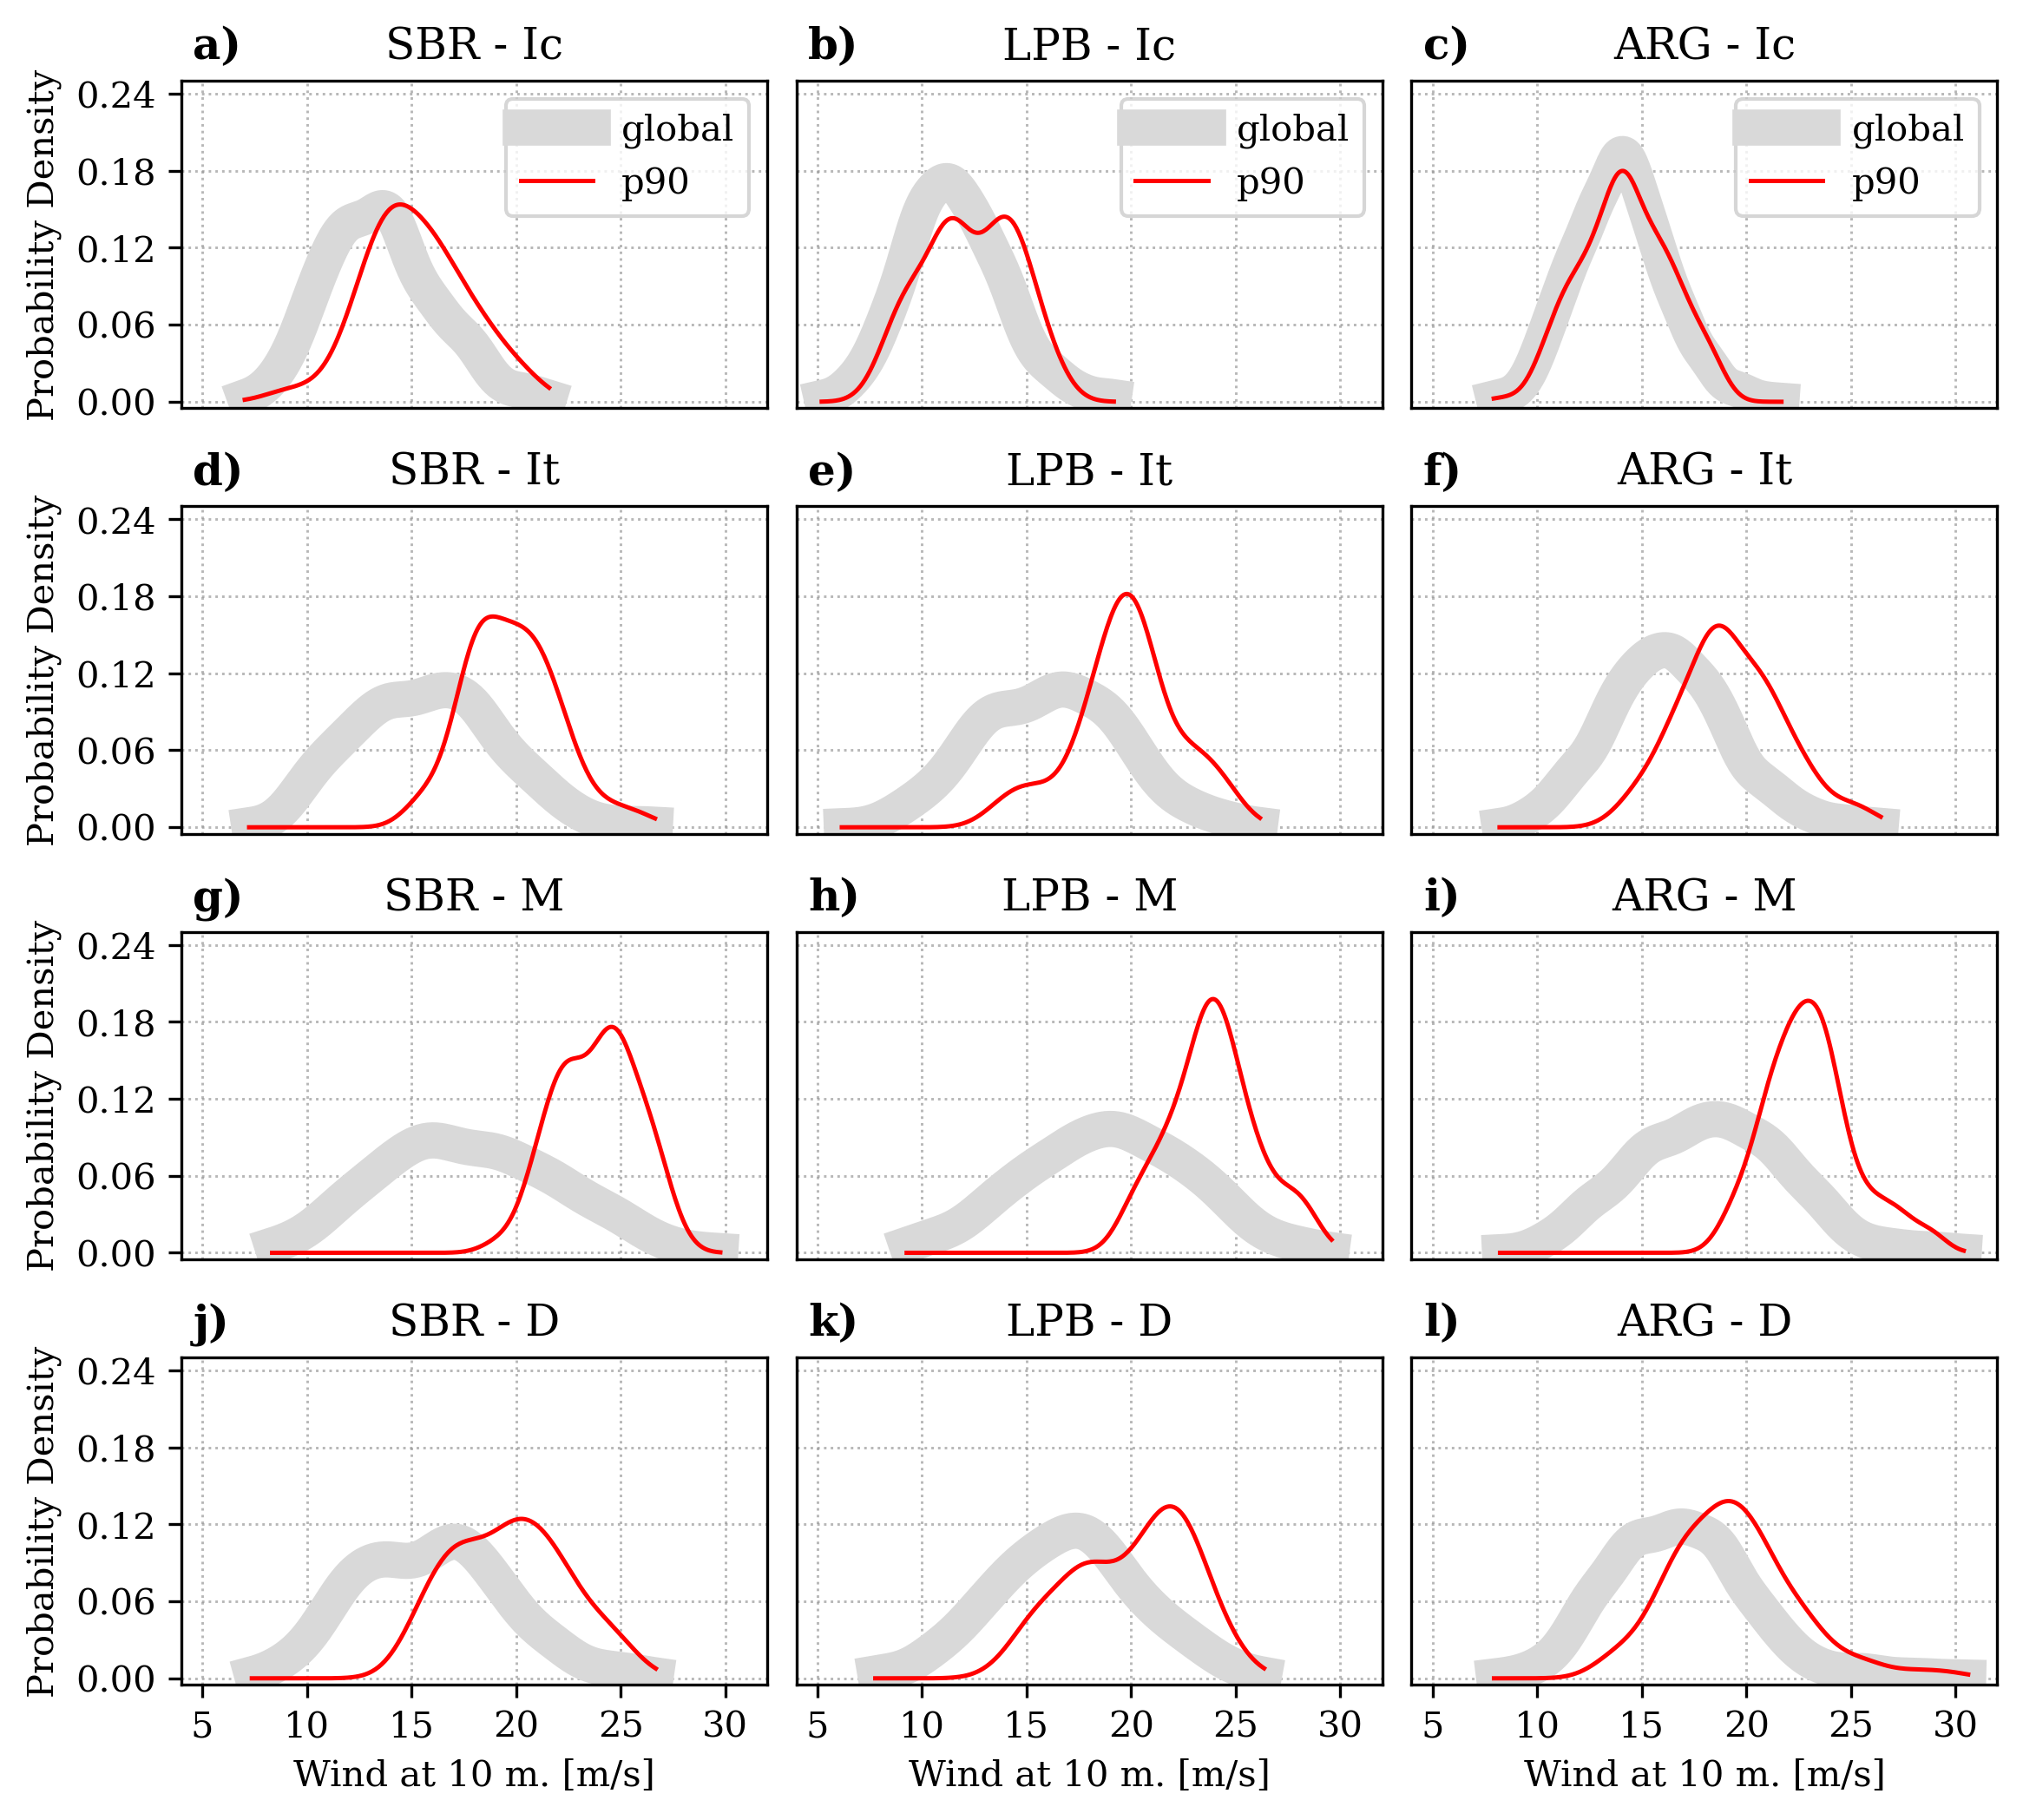
\includegraphics[width=\textwidth]{images/w10/PDF_wind10_sigma025.png}
\caption[PDF de magnitudes máximas de vento a 10 metros]{Funções de densidade de probabilidade (PDF) para as magnitudes máximas de vento a 10 metros. As colunas indicam a região de ciclogênese (SBR, LPB, ARG) e as fileiras a evolução através das fases do ciclo de vida (Ic, It, M, D). Contrasta-se a população global (referência, sombreado cinza) com os subconjuntos definidos por percentis dos máximos de vorticidade relativa em 850 hPa alcançados em seu ciclo vital: $p90$ (sistemas intensos, linha vermelha).}
\label{fig:pdf_wind10}
\end{figure}

A Figura \ref{fig:pdf_wind10} apresenta as funções de densidade de probabilidade que descrevem a distribuição estatística dos máximos de vento em superfície a 10 metros. 
Esses valores foram extraídos sistematicamente do domínio lagrangiano como se explica em \ref{subsec:extraccion_pdf}. 
Este enfoque é consistente com metodologias prévias aplicadas no Atlântico Sudoeste, como a de \citet{cardoso2022synoptic}, e responde à evolução física do sistema; como demonstrou \citet{simmonds2000size}, o raio dos ciclones em superfície tende a incrementar-se sistematicamente à medida que evoluem para a maturidade em ambos os hemisférios. 
Além disso, esta grande extensão é crítica para capturar o forçante sobre o oceano; \citet{sasaki2021intraseasonal} ressaltaram o papel fundamental desses ciclones na variabilidade intra-sazonal das ondas no Atlântico Sul ocidental, onde a configuração do vento em superfície determina a transferência de energia para o estado do mar. 
Portanto, o domínio adotado permite integrar de forma robusta tanto o núcleo do sistema como os ventos associados.
A amostra encontra-se estratificada por região de ciclogênese (SBR, LPB, ARG) e sua evolução é avaliada transversalmente ao longo das quatro fases de desenvolvimento (Ic, It, M, D). A análise contrasta a População Global de referência contra o subconjunto de sistemas intensos ($p90$).

Durante a fase incipiente (Ic; painéis a, b e c), tanto a População Global como o subconjunto $p90$ apresentam distribuições unimodais estreitas parcialmente sobrepostas, com frequências máximas concentradas no intervalo de 10 a 17 m/s. À medida que os sistemas evoluem independentemente para as fases de intensificação (It; painéis d, e e f) e maturidade (M; painéis g, h e i), torna-se evidente a divergência entre os grupos: a curva do subconjunto $p90$ desloca-se drasticamente para a direita, alcançando na fase M um pico modal no intervalo de 20 a 22 m/s e caudas estendendo-se até os 30 m/s, enquanto a População Global mantém seu máximo ao redor dos 12--15 m/s com uma distribuição mais estreita e simétrica. Regionalmente, na etapa de maturidade da SBR (g), o $p90$ exibe um pico de densidade ($\sim$0,18) e acotado em altas velocidades; LPB (h) apresenta igualmente um deslocamento para velocidades maiores, embora com um pico mais baixo e distribuição mais estendida ($\sim$0,07), enquanto ARG (i) mostra a distribuição mais ampla e aplanada das três regiões, evidenciando uma maior heterogeneidade na intensidade de seus sistemas. Finalmente, na fase de decadência (D; painéis j, k e l), as curvas do subconjunto $p90$ recuam levemente para magnitudes menores e aumentam sua dispersão, preservando no entanto uma separação inconfundível em relação aos sistemas mais fracos.

A máxima separação das distribuições na fase de maturidade reflete o momento em que os ciclones intensos ($p90$) expressam seu pleno potencial dinâmico, alcançando seu mínimo absoluto de vorticidade relativa a 850 hPa e maximizando o gradiente horizontal de pressão superficial. A marcada diferença em relação à População Global evidencia que esses vórtices possuem, desde sua gênese, um ambiente ou forçante mais instável que culmina em campos de vento substancialmente mais severos que o desenvolvimento padrão da climatologia média.

As variações interregionais refletem distintos forçamentos físicos predominantes. Tal como sustenta \citet{gramcianinov2024early}, os sistemas nas regiões SBR e LPB alcançam intensidades de vento mais extremas devido à forte influência de processos termodinâmicos em níveis baixos — como a advecção quente e a convergência de umidade de origem oceânica e continental —, fatores que os modelos de alta resolução logram representar com maior fidelidade. 
Esta dependência termodinâmica ilustra-se na análise do ciclone Raoni realizada por \citet{reboita2022from}, onde evidenciou-se que os fluxos turbulentos de calor sensível e latente desde o oceano, junto com o transporte de umidade continental pelos ventos, foram decisivos para fortalecer o sistema e organizar a convecção. 
% Asimismo, experimentos numéricos confirman que la representación precisa de estos intercambios de calor en superficie es esencial para capturar la intensificación de los vientos en niveles bajos. 
Este aspecto termodinâmico é analisado por \citet{russo2025impacts}, os quais sustentam que, embora a ciclogênese inicial dependa frequentemente de processos dinâmicos de níveis altos, a injeção massiva de umidade e fluxos de calor latente resulta fundamental durante as fases de intensificação e maturidade.

Enquanto isso, em ARG, a dinâmica baroclínica clássica do frente polar e a perturbação topográfica dos Andes geram respostas cinemáticas mais variáveis e distribuições mais aplanadas. 
De acordo com \citet{gan1994influence}, a cordilheira induz severas distorções espaciais no fluxo de níveis baixos, enquanto \citet{vera2002cold} detalham a profunda modificação na estrutura tridimensional das ondas ao cruzar o relevo andino. 
Esta modulação orográfica explica a maior heterogeneidade e irregularidade geométrica no campo de ventos superficiais para os sistemas gerados nesta região.

A quantificação dessas distribuições permite comparar objetivamente como evoluem as magnitudes mais prováveis e a extensão dos valores entre ciclones de distinta gênese. 
Ao confirmar que os ciclones classificados dinamicamente como intensos $p90$ se separam sistematicamente da população à medida que amadurecem, valida-se a pertinência da classificação baseada em vorticidade. 
Na fase de maturidade, o subgrupo $p90$ desloca sua maior probabilidade para os 23 m/s, o que representa um incremento de aproximadamente 50\% na intensidade do vento da população global. 
As caudas nas distribuições $p90$ alcançam magnitudes críticas de até 30 m/s. Este deslocamento coincide com os registros documentados por \citet{padilhareinke2026characterization} e \citet{gramcianinov2020analysis} para os eventos severos do Atlântico Sul. 
\citet{padilhareinke2026characterization} reportam uma intensidade média de vento a 10 metros de 70,0 km/h ($\approx$ 19,4 m/s), com um limiar para eventos intensos $p90$ de 84,4 km/h ($\approx$ 23,4 m/s) e magnitudes extremas que alcançam até 113,21 km/h ($\approx$ 31,4 m/s) nas caudas da distribuição. 
Esses intervalos são consistentes com o documentado por \citet{gramcianinov2020analysis}, os quais reportam, para o inverno austral (JJA, do inglês), velocidades máximas médias de entre 21,2 $\pm$ 4,8 m/s e 23,4 $\pm$ 4,8 m/s, com valores do percentil 90 de entre 27,3 e 30,2 m/s e do percentil 95 de até 32,1 m/s em bases de dados de alta resolução como CFSR/CFSv2 (do inglês). 
Desde uma perspectiva analítica, o observado no Hemisfério Norte por \citet{corner2025classification}, os quais empregam um método de classificação de ciclones distinto, identifica que o grupo dos ciclones mais fracos apresenta uma moda na velocidade do vento a 10 metros de 12,5 m/s; em contraste, ciclones mais intensos alcançam os 22,5 m/s. 
As caudas nas distribuições deste subconjunto $p90$ alcançam magnitudes críticas de até 32 m/s.
% , lo que confirma que estos sistemas mantienen consistentemente sus valores de viento por encima del umbral de los 20 m/s.

Como sublinha \citet{gramcianinov2023impact}, identificar precocemente sistemas intensos resulta indispensável, já que esses ventos anômalos são os forçantes para eventos associados que supõem um risco direto para as regiões costeiras e marítimas.

% ==============================================================================
% SECCIÓN PRINCIPAL: KDE ESPACIAL DE VIENTO A 10 METROS
% ==============================================================================
%
\section{Distribuição espacial de máximos (KDE)}
% $$$$
\subsection{População Global}\label{sec:kde_espacial_global}

\begin{figure}[htbp]
\centering
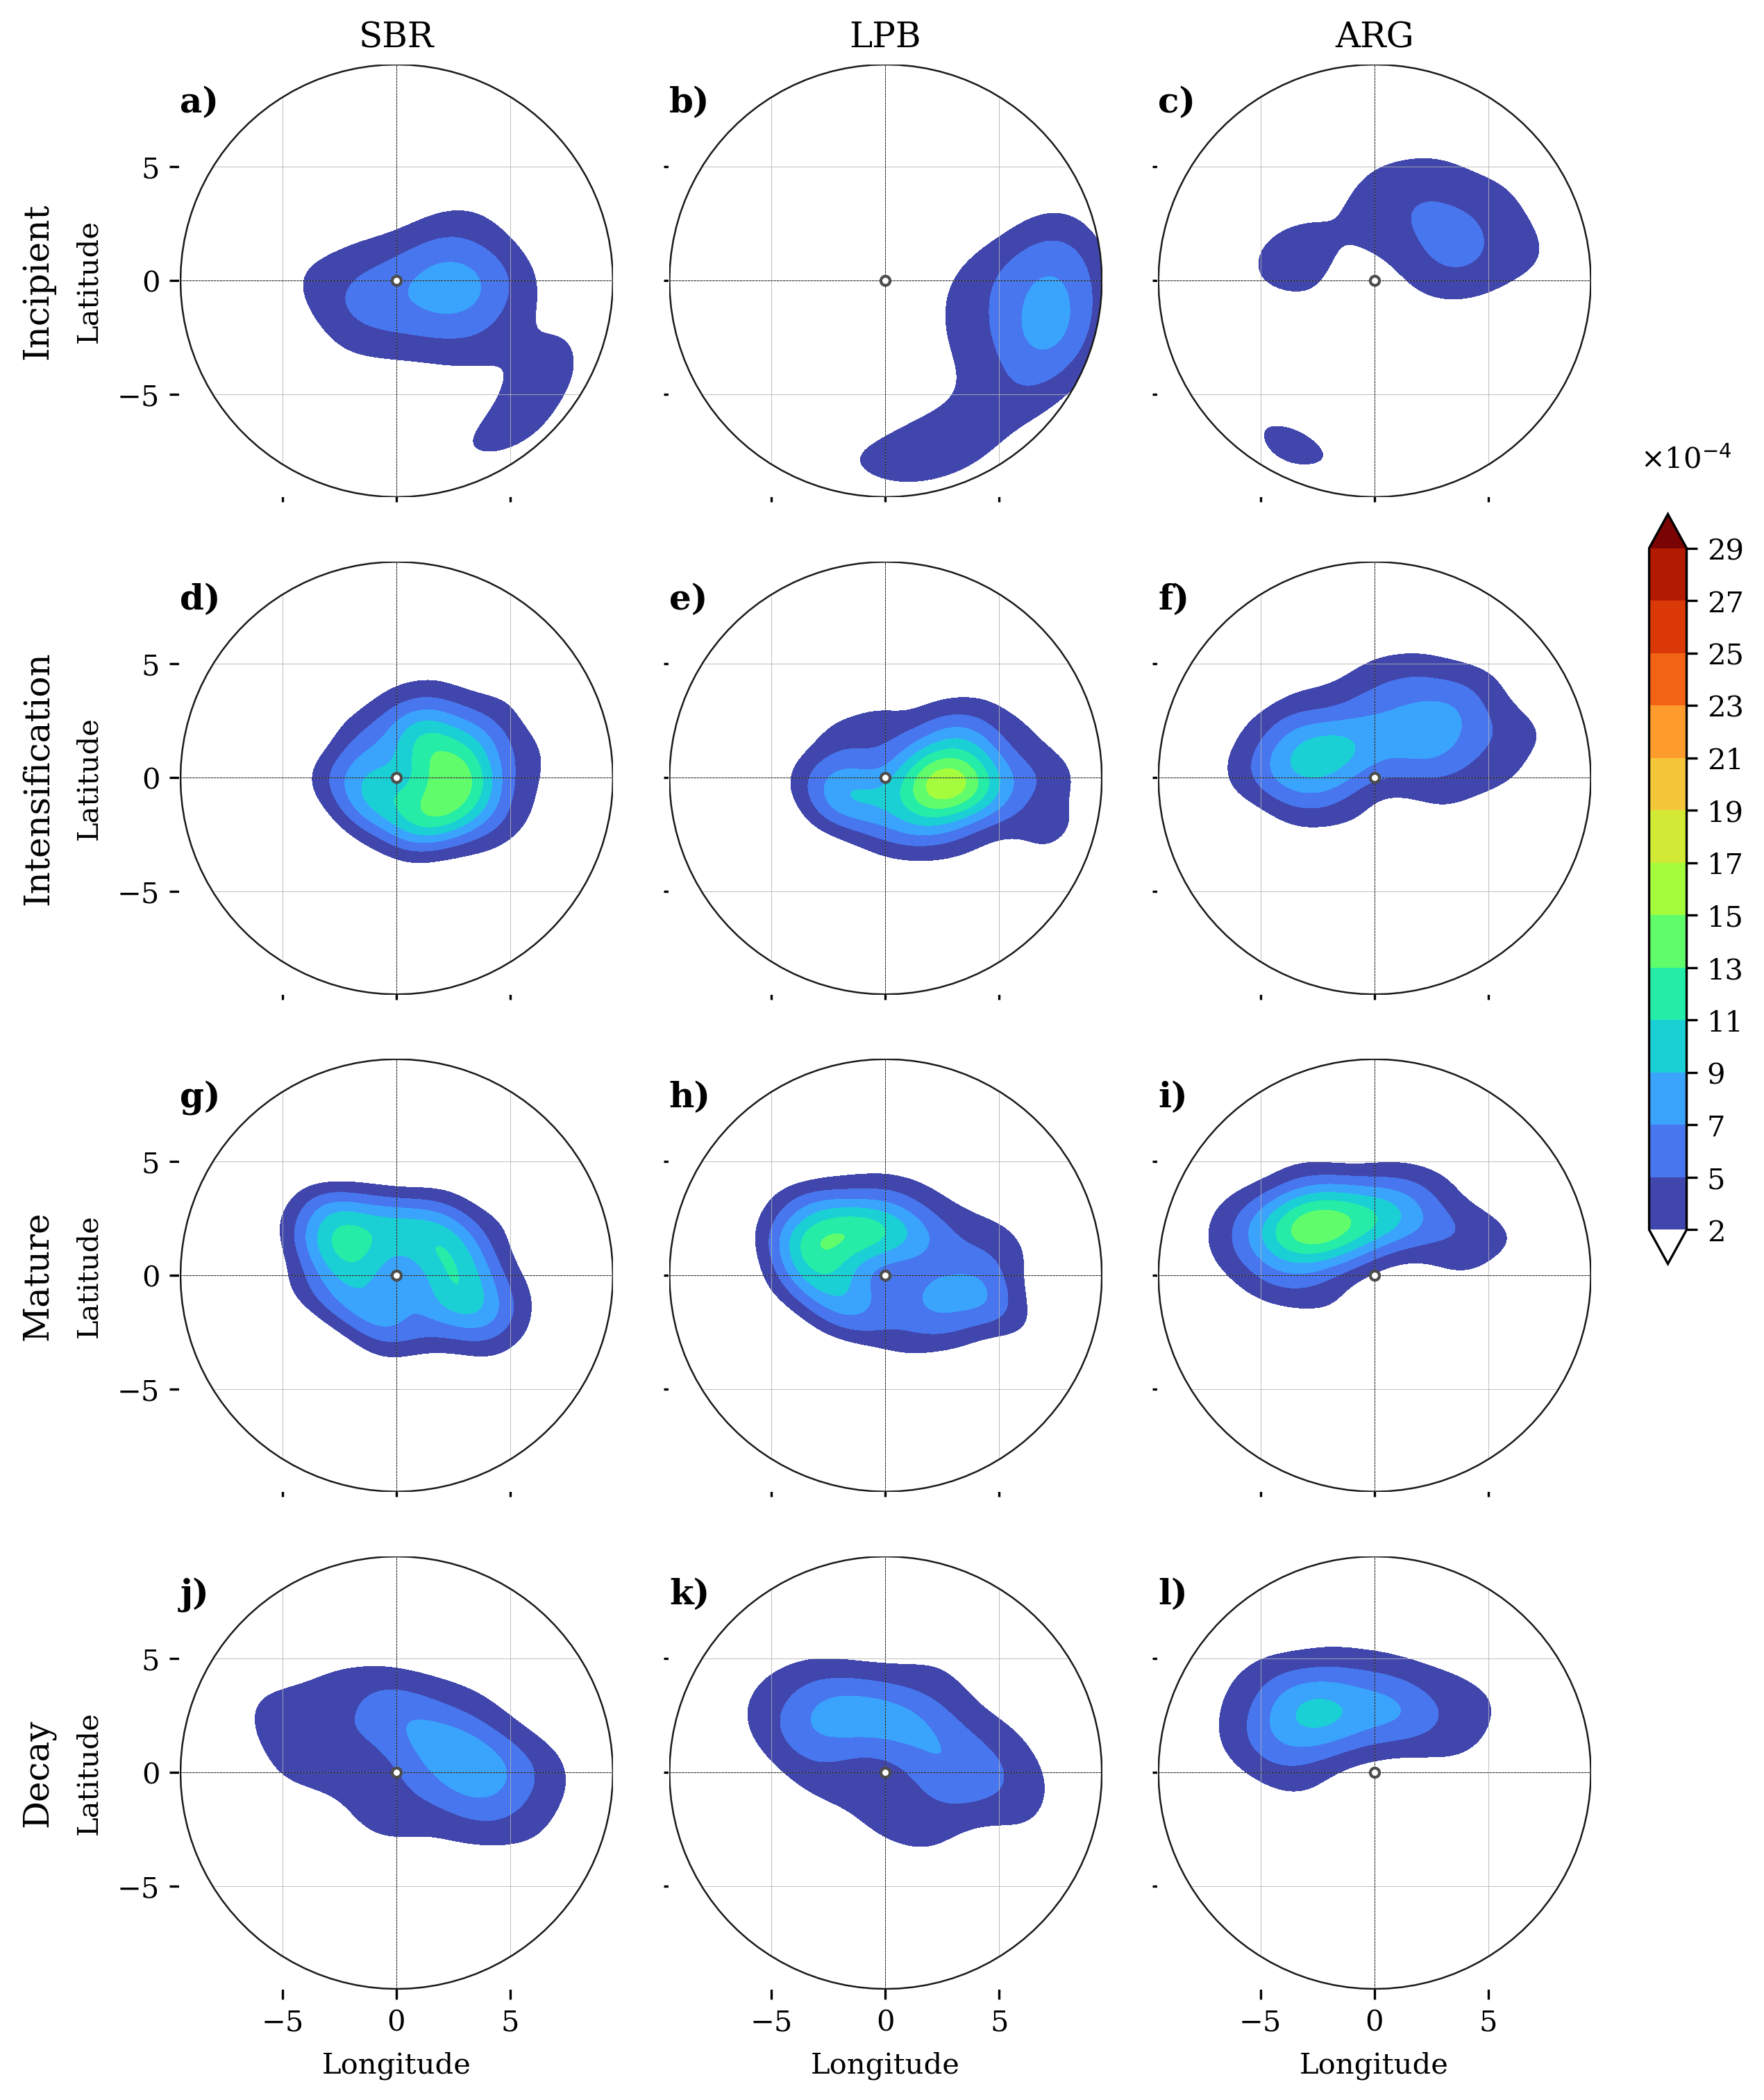
\includegraphics[width=\textwidth]{images/w10/kde_wind10_global_fasesxreg.png}
\caption[PDF espacial de vento máximo a 10 metros - População Global]{Estimação de densidade espacial bidimensional da localização dos máximos de magnitude de vento a 10 metros para a População Global. As colunas separam as regiões de ciclogênese (SBR, LPB, ARG) e as fileiras indicam as fases evolutivas (Ic, It, M, D). O domínio lagrangiano está centrado no ciclone ($0^\circ, 0^\circ$).}
\label{fig:kde_wind_global}
\end{figure}

A Figura~\ref{fig:kde_wind_global} apresenta o campo de densidade espacial sobre o domínio lagrangiano de $20^\circ \times 20^\circ$ previamente definido. 
Em nível global, a distribuição caracteriza-se por ser ampla, difusa e com gradientes de probabilidade suaves. 
Nas fases iniciais (Ic; painéis a, b e c), as zonas de máxima densidade abrangem áreas extensas que não definem uma estrutura simétrica ao redor do centro do ciclone. 
Esta falta de organização inicial é consistente com a alta variabilidade na intensidade dos sistemas descrita por \citet{reboita2010south}, o qual destaca uma abundante ocorrência de ciclones que iniciam com uma estrutura fraca ou rasa. 
Em fases precoces, esses sistemas costumam apresentar circulações assimétricas, coincidindo com \citet{gozzo2017climatology} sobre a dificuldade desses vórtices para organizar uma circulação fechada.

À medida que os sistemas avançam para a maturidade (M; painéis g, h e i), observa-se uma leve preferência de localização no quadrante noroeste, mantendo diferenças posicionais entre regiões. 
Como sugere \citet{dossantos2023response}, esta evolução espacial assimétrica está ligada às zonas baroclínicas, onde os máximos gradientes térmicos horizontais interagem com os jatos na alta troposfera.
Nesta etapa, a densidade máxima em ARG (i) alcança valores de $\approx$\,19--21 $\times 10^{-4}$, enquanto SBR (g) e LPB (h) alcançam maior densidade em áreas mais restritas, indicando um foco mais recorrente para a localização de ventos máximos. 
Este contraste regional responde a forçantes distintos: enquanto os sistemas em ARG estão modulados principalmente pela advecção térmica, a maior concentração em SBR e LPB favorece-se pela advecção de ar quente e úmido junto ao desenvolvimento de baixas orográficas em etapas iniciais \citep{gramcianinov2019properties, cardoso2022synoptic}.
Esta alta dispersão espacial é inerente ao uso de um catálogo massivo onde os sistemas variam desde configurações fracas até atípicas. 
Como assinala \citet{sinclair1994objective}, os métodos de identificação baseados em vorticidade capturam um espectro amplo que inclui numerosos ciclones fracos, móveis e de menor duração. 
Fisicamente, quando a interação baroclínica é fraca, o fluxo sinóptico de níveis médios ou altos domina a circulação e o sistema é governado por anomalias na alta troposfera que não logram consolidar um acoplamento profundo, modificando a localização do vento máximo em função de gradientes de pressão transitórios \citep{hoskins2005new}.

A caracterização desta dispersão demonstra que, na população geral, o máximo de vento pode ocorrer em um raio muito amplo e variável. 
Esta heterogeneidade justifica metodologicamente a estratificação por intensidade, respaldada por \citet{corner2025classification} e \citet{eisenstein2023identification}, os quais destacam que a diversidade desses sistemas exige classificá-los para isolar os eventos severos. 
Embora esta estratificação seja habitual no Hemisfério Norte, sua aplicação sistemática no Hemisfério Sul permanece como necessidade crítica. 
O contraste contra esta linha de base revela imediatamente a organização geométrica dos sistemas intensos, cuja arquitetura espacial se examina a seguir.

\subsection{Subconjunto de ciclones intensos $p90$}\label{sec:kde_espacial_p90}

\begin{figure}[htbp]
\centering
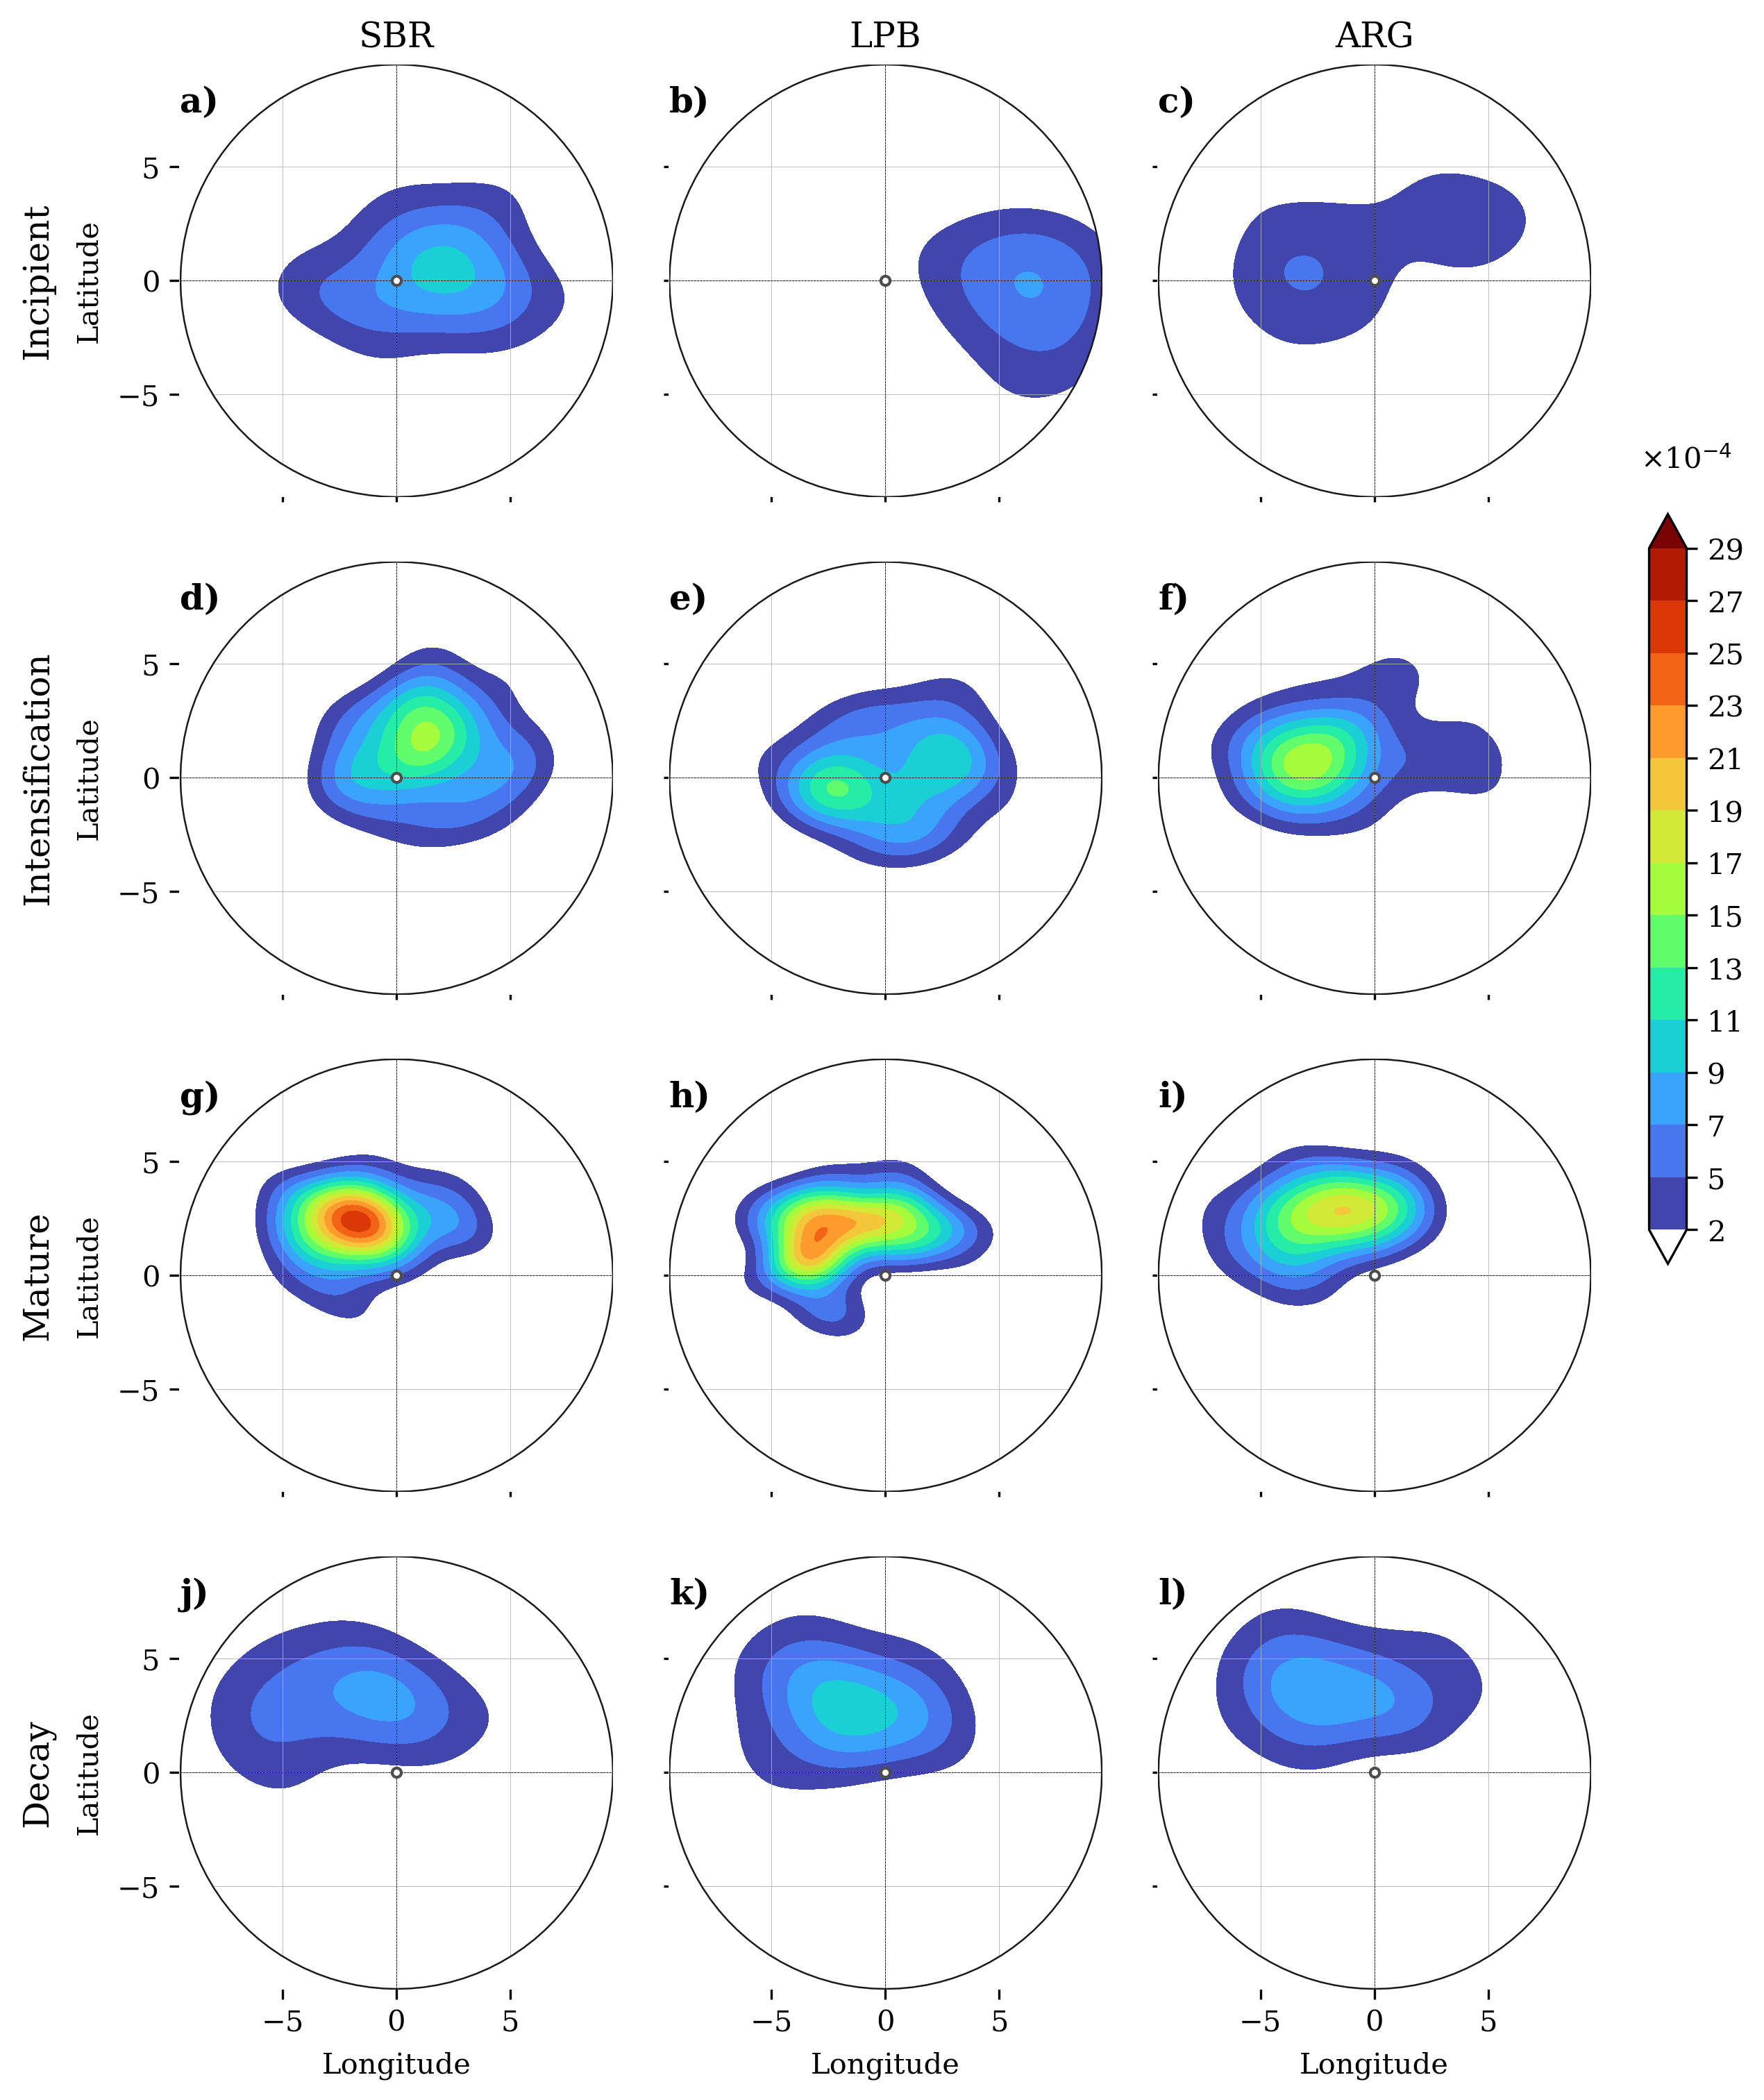
\includegraphics[width=\textwidth]{images/w10/kde_wind10_p90_fasesxreg.png}
\caption[PDF espacial de vento máximo a 10 metros - Subconjunto p90]{Estimação de densidade espacial bidimensional da localização dos máximos de magnitude de vento a 10 metros para o subconjunto de ciclones intensos. O formato, domínio lagrangiano, fases evolutivas e escala de densidade ($10^{-4}$) são idênticos aos apresentados na Figura~\ref{fig:kde_wind_global} para permitir a comparação estrutural direta das assimetrias de densidade.}
\label{fig:kde_wind_p90}
\end{figure}

Ao contrastar esta linha de base contra o subconjunto de sistemas intensos ($p90$), a reorganização espacial resulta drástica. A Figura~\ref{fig:kde_wind_p90} revela que a arquitetura dos ventos máximos deixa de ser difusa para configurar um núcleo de alta densidade marcadamente concentrado no quadrante noroeste durante a fase de maturidade (M; painéis g, h e i), localizado aproximadamente a $-1^{\circ}$ a $-2^{\circ}$ de longitude e entre $+1^{\circ}$ e $+2^{\circ}$ de latitude relativa ao centro. As magnitudes de densidade alcançadas em SBR (g) são particularmente extremas (valores entre 23 e $27 \times 10^{-4}$, tons laranja--avermelhados), enquanto LPB (h) alcança valores de $\approx$\,23--25\,$\times 10^{-4}$, denotando uma recorrência espacial para a localização dos ventos máximos. 
Por sua parte, ARG (i) exibe igualmente uma concentração em relação à população global, embora com um núcleo de densidade comparativamente menor e ligeiramente mais disperso. 
Na fase de decadência (D; painéis j, k e l), este núcleo assimétrico mantém-se ancorado no setor noroeste, diferentemente do comportamento na população global durante esta etapa.

Esta hiperconcentração no quadrante noroeste (Hemisfério Sul) constitui a assinatura espacial cinemática dos ciclones profundos maduros. Como foi documentado para o Hemisfério Norte (quadrante sudoeste) por \citet{clark2005sting} e \citet{han2025system}, os sistemas extratropicais mais intensos empacotam seus ventos extremos no setor posterior, associados especificamente à zona de fratura frontal e ao desenvolvimento de intensas correntes em jato de níveis baixos (\textit{sting jet} ou cinta transportadora fria). 
Esta distinção dinâmica é fundamental, já que como precisam \citet{martinez2014cold}, os ventos mais intensos na retaguarda do núcleo costumam ser o produto combinado da cinta transportadora fria (CCB, do inglês) e os \textit{sting jets} (SJ, do inglês) transitórios. 
Curiosamente, embora \citet{stankovic2025surface} demonstrem que os extremos absolutos de vento em superfície em escala global tendem a ser maiores nos oceanos do Hemisfério Norte devido a uma maior baroclinicidade, os valores registrados nas caudas da distribuição $p90$ da região alcançam valores similares.

Ao aplicar o efeito espelho produto da circulação ciclônica inversa entre hemisférios, a configuração dinâmica do setor posterior corresponderia espacialmente ao quadrante noroeste. 
Fisicamente, a consolidação deste núcleo extremo responde a processos de transferência de quantidade de movimento: nas imediações do frente frio desenvolvem-se intensas correntes descendentes que transportam o momento horizontal da alta troposfera para a camada limite \citep{hyeok2024extrem}. 
No entanto, deve considerar-se que os dados de reanálise ERA5 podem subestimar a intensidade real do vento devido a limitações de resolução. 
\citet{priestley2022improved} documentaram sistematicamente esta limitação, demonstrando que a incapacidade dos modelos globais para resolver de forma explícita as estruturas de mesoescala dentro da tempestade conduz a uma subestimação inerente das magnitudes extremas. 
Somado a isto, como demonstram \citet{gentile2023observed}, os jatos da cinta transportadora fria (CCBb, do inglês) em ciclones maduros estão associados com camadas limite significativamente mais profundas, potencializadas pela instabilidade que gera o ar frio ao circular sobre águas oceânicas relativamente quentes; isto induz fluxos de calor positivos que facilitam uma mistura vertical descendente altamente eficiente de ar de alta velocidade para a superfície, manifestando-se no KDE como um empacotamento localizado a 10 metros, setor onde o CCBb constitui o principal motor de ventos a pesar de modelos como o ERA5 tenderem a subestimar suas intensidades em aproximadamente 4,5~m~s$^{-1}$.

As diferenças interregionais observadas na Figura~\ref{fig:kde_wind_p90} — particularmente a maior concentração em SBR e LPB em relação a ARG — respaldam este marco dinâmico. Por um lado, \citet{reboita2018extratropical} destaca que o Atlântico Sudoeste é um ambiente onde as interações diabáticas e os fortes fluxos de calor latente oceano-atmosfera fomentam a rápida intensificação dos sistemas. Conectando esses processos térmicos com uma zonificação específica, \citet{gramcianinov2023impact} assinala que os ciclones originados particularmente em SBR e LPB capitalizam essas condições para gerar desenvolvimentos de tipo explosivo, empacotando o momento cinético em um setor espacial muito estreito. Pelo contrário, em ARG, a dinâmica baroclínica clássica do frente polar e a perturbação topográfica dos Andes geram estruturas marginalmente mais alongadas que deixarão as localizações dos máximos de vento menos concentradas.

A quantificação desta concentração demonstra que o grau de severidade de um ciclone predetermina seu padrão espacial. Os sistemas intensos originados no Atlântico Sul concentrarão quase invariavelmente seus máximos de vento a 10 metros em um raio e quadrante particular em relação ao seu centro. Tal como destaca \citet{dalanhese2023new} para o litoral sul-americano, esta previsibilidade geométrica é uma ferramenta importante para conhecer a espacialidade das possíveis afetações que possam ocorrer durante esses eventos severos.

% ==============================================================================
% SECCIÓN: PATRONES DOMINANTES DE VARIABILIDAD (EOF) - VIENTO A 10 METROS
% ==============================================================================
\section{Organização estrutural: Análise EOF}\label{sec:eof_wind10}
\subsection{Fracionamento de variância}\label{sec:var_exp_wind10}

\begin{figure}[!ht]
\centering
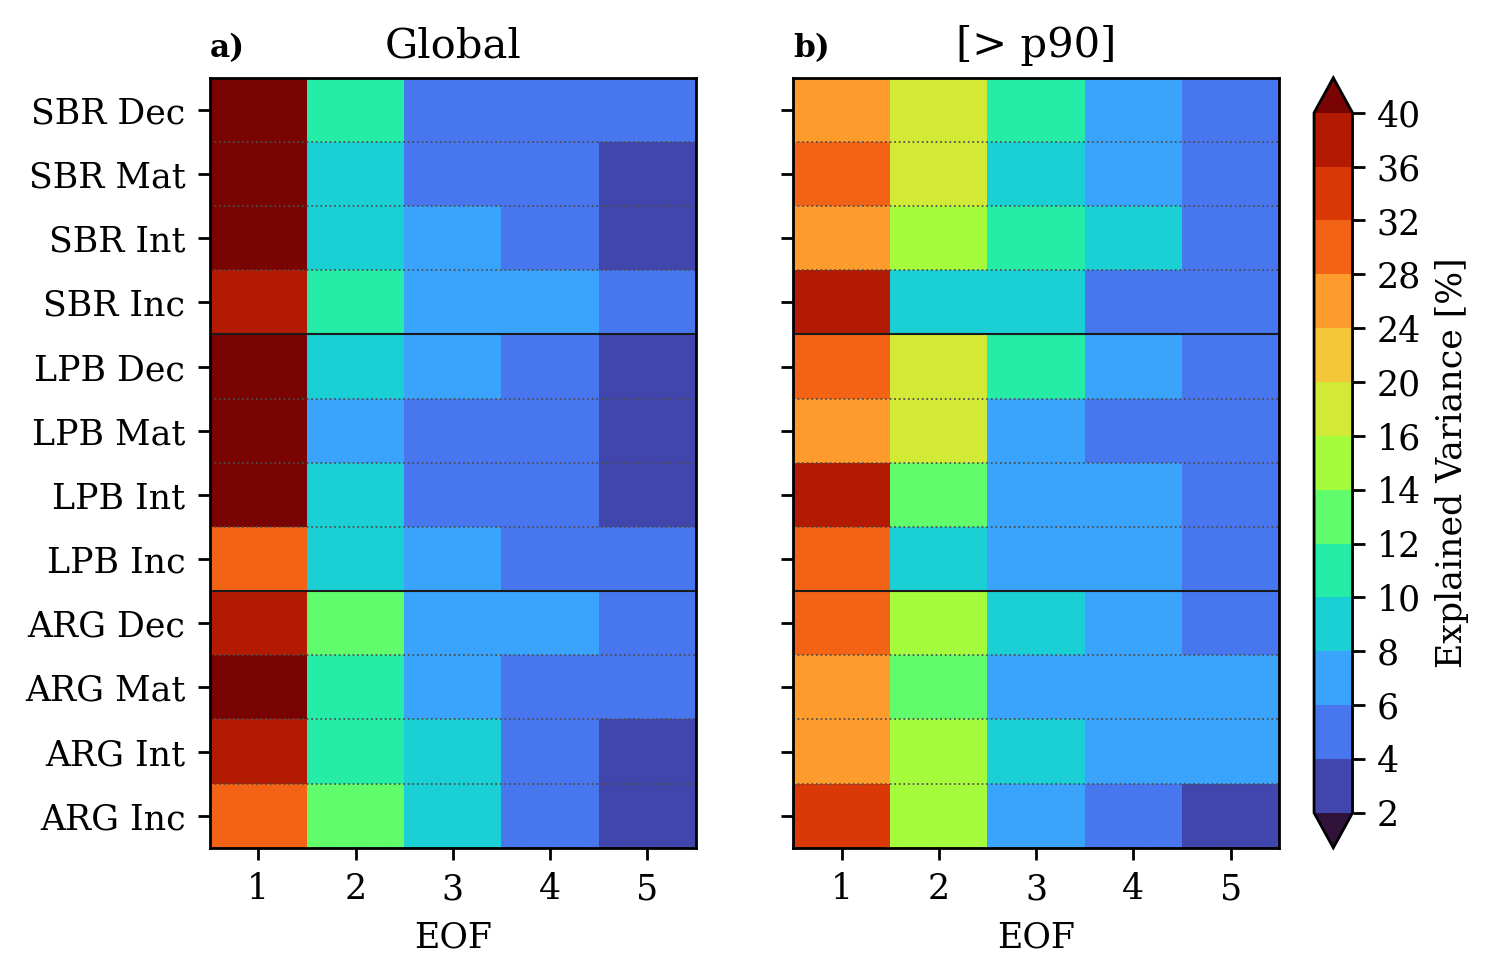
\includegraphics[width=0.8\textwidth]{images/w10/all_expvar_wind10_mean2times.png} 
\caption[Variância explicada pelos primeiros cinco modos (EOF1--EOF5) de vento a 10 m]{Fracionamento da variância espacial total contida nos primeiros cinco modos dominantes (EOF1 a EOF5) do vento a 10 metros. Contrasta-se a distribuição da variância da População Global frente ao subconjunto de intensidade $p90$ ao longo do ciclo de vida para cada região de ciclogênese.}
\label{fig:var_exp_wind10}
\end{figure}

% ¿Qué es?
A Figura \ref{fig:var_exp_wind10} sintetiza o fracionamento da variância espacial distribuída nos primeiros cinco modos ortogonais (EOF1 a EOF5) do campo de vento superficial. 
Contrasta-se o comportamento da População Global de referência frente aos estratos de distinta intensidade dinâmica intrínseca ($p90$) ao longo das fases evolutivas.

% ¿Cómo es?
A análise revela uma divergência drástica na distribuição da variância entre a População Global e o subconjunto $p90$. 
Na População Global, o modo EOF1 exerce um domínio avassalador, capturando até 57,1\% (LPB) e 57,4\% (SBR) da variância durante a fase de maturidade, que é onde o domínio do EOF1 resulta mais pronunciado nessas regiões. 
Isto gera uma queda abrupta entre o primeiro modo e os modos de ordem superior (EOF2 a EOF5), os quais retêm porções marginais de variância explicada, confirmando que na climatologia média a dinâmica do vento está governada por um padrão espacial dominante. 
Pelo contrário, no subconjunto $p90$, a concentração de variância em EOF1 reduz-se drasticamente: o EOF1 não logra superar os 37,6\% de representatividade, registrando mínimos de até 25,4\% durante a intensificação em ARG. 
Consequentemente, a variância do $p90$ reparte-se e aplana entre múltiplos modos, inflando a importância relativa dos modos secundários (EOF2 e EOF3).

A alta concentração de energia em um único modo (EOF1) para a População Global corrobora que os ciclones típicos são governados por um gradiente de grande escala imposto pelo fluxo sinóptico de fundo. 
No entanto, o aplanamento da variância nos eventos $p90$ confirma estatisticamente a fragmentação multiescalar. 
Tal como estabelece a teoria matemática de \citet{hannachi2007empirical}, um espectro de autovalores mais plano é o indicador de que a energia de um sistema distribuiu-se entre múltiplos modos competitivos. 
Ao intensificar-se, o vórtice gera perturbações internas não lineares: frentes excepcionalmente ativas, correntes em jato de baixos níveis e seclusões térmicas. 
Estas estruturas de mesoescala competem entre si pela energia cinética do campo, obrigando a decomposição matemática a utilizar múltiplas dimensões ortogonais (EOF2--EOF5) para poder reconstruir o caos cinemático do ciclone.

Esta métrica constitui uma demonstração quantitativa de que a severidade não equivale a um simples escalonamento linear de um ciclone ordinário. 
Concluir que os eventos $p90$ requerem múltiplas dimensões espaciais para serem explicados demonstra que parametrizar ventos destrutivos assumindo os padrões simples da população média subestimará sistematicamente a agressividade, a natureza assimétrica e a localização dos máximos.

% ==============================================================================
\subsection{Padrões espaciais dominantes (EOF1)}\label{subsec:eof1_wind10}
% ==============================================================================
\subsubsection{População Global}\label{subsubsec:eof1_wind10_global}

\begin{figure}[htbp]
\centering
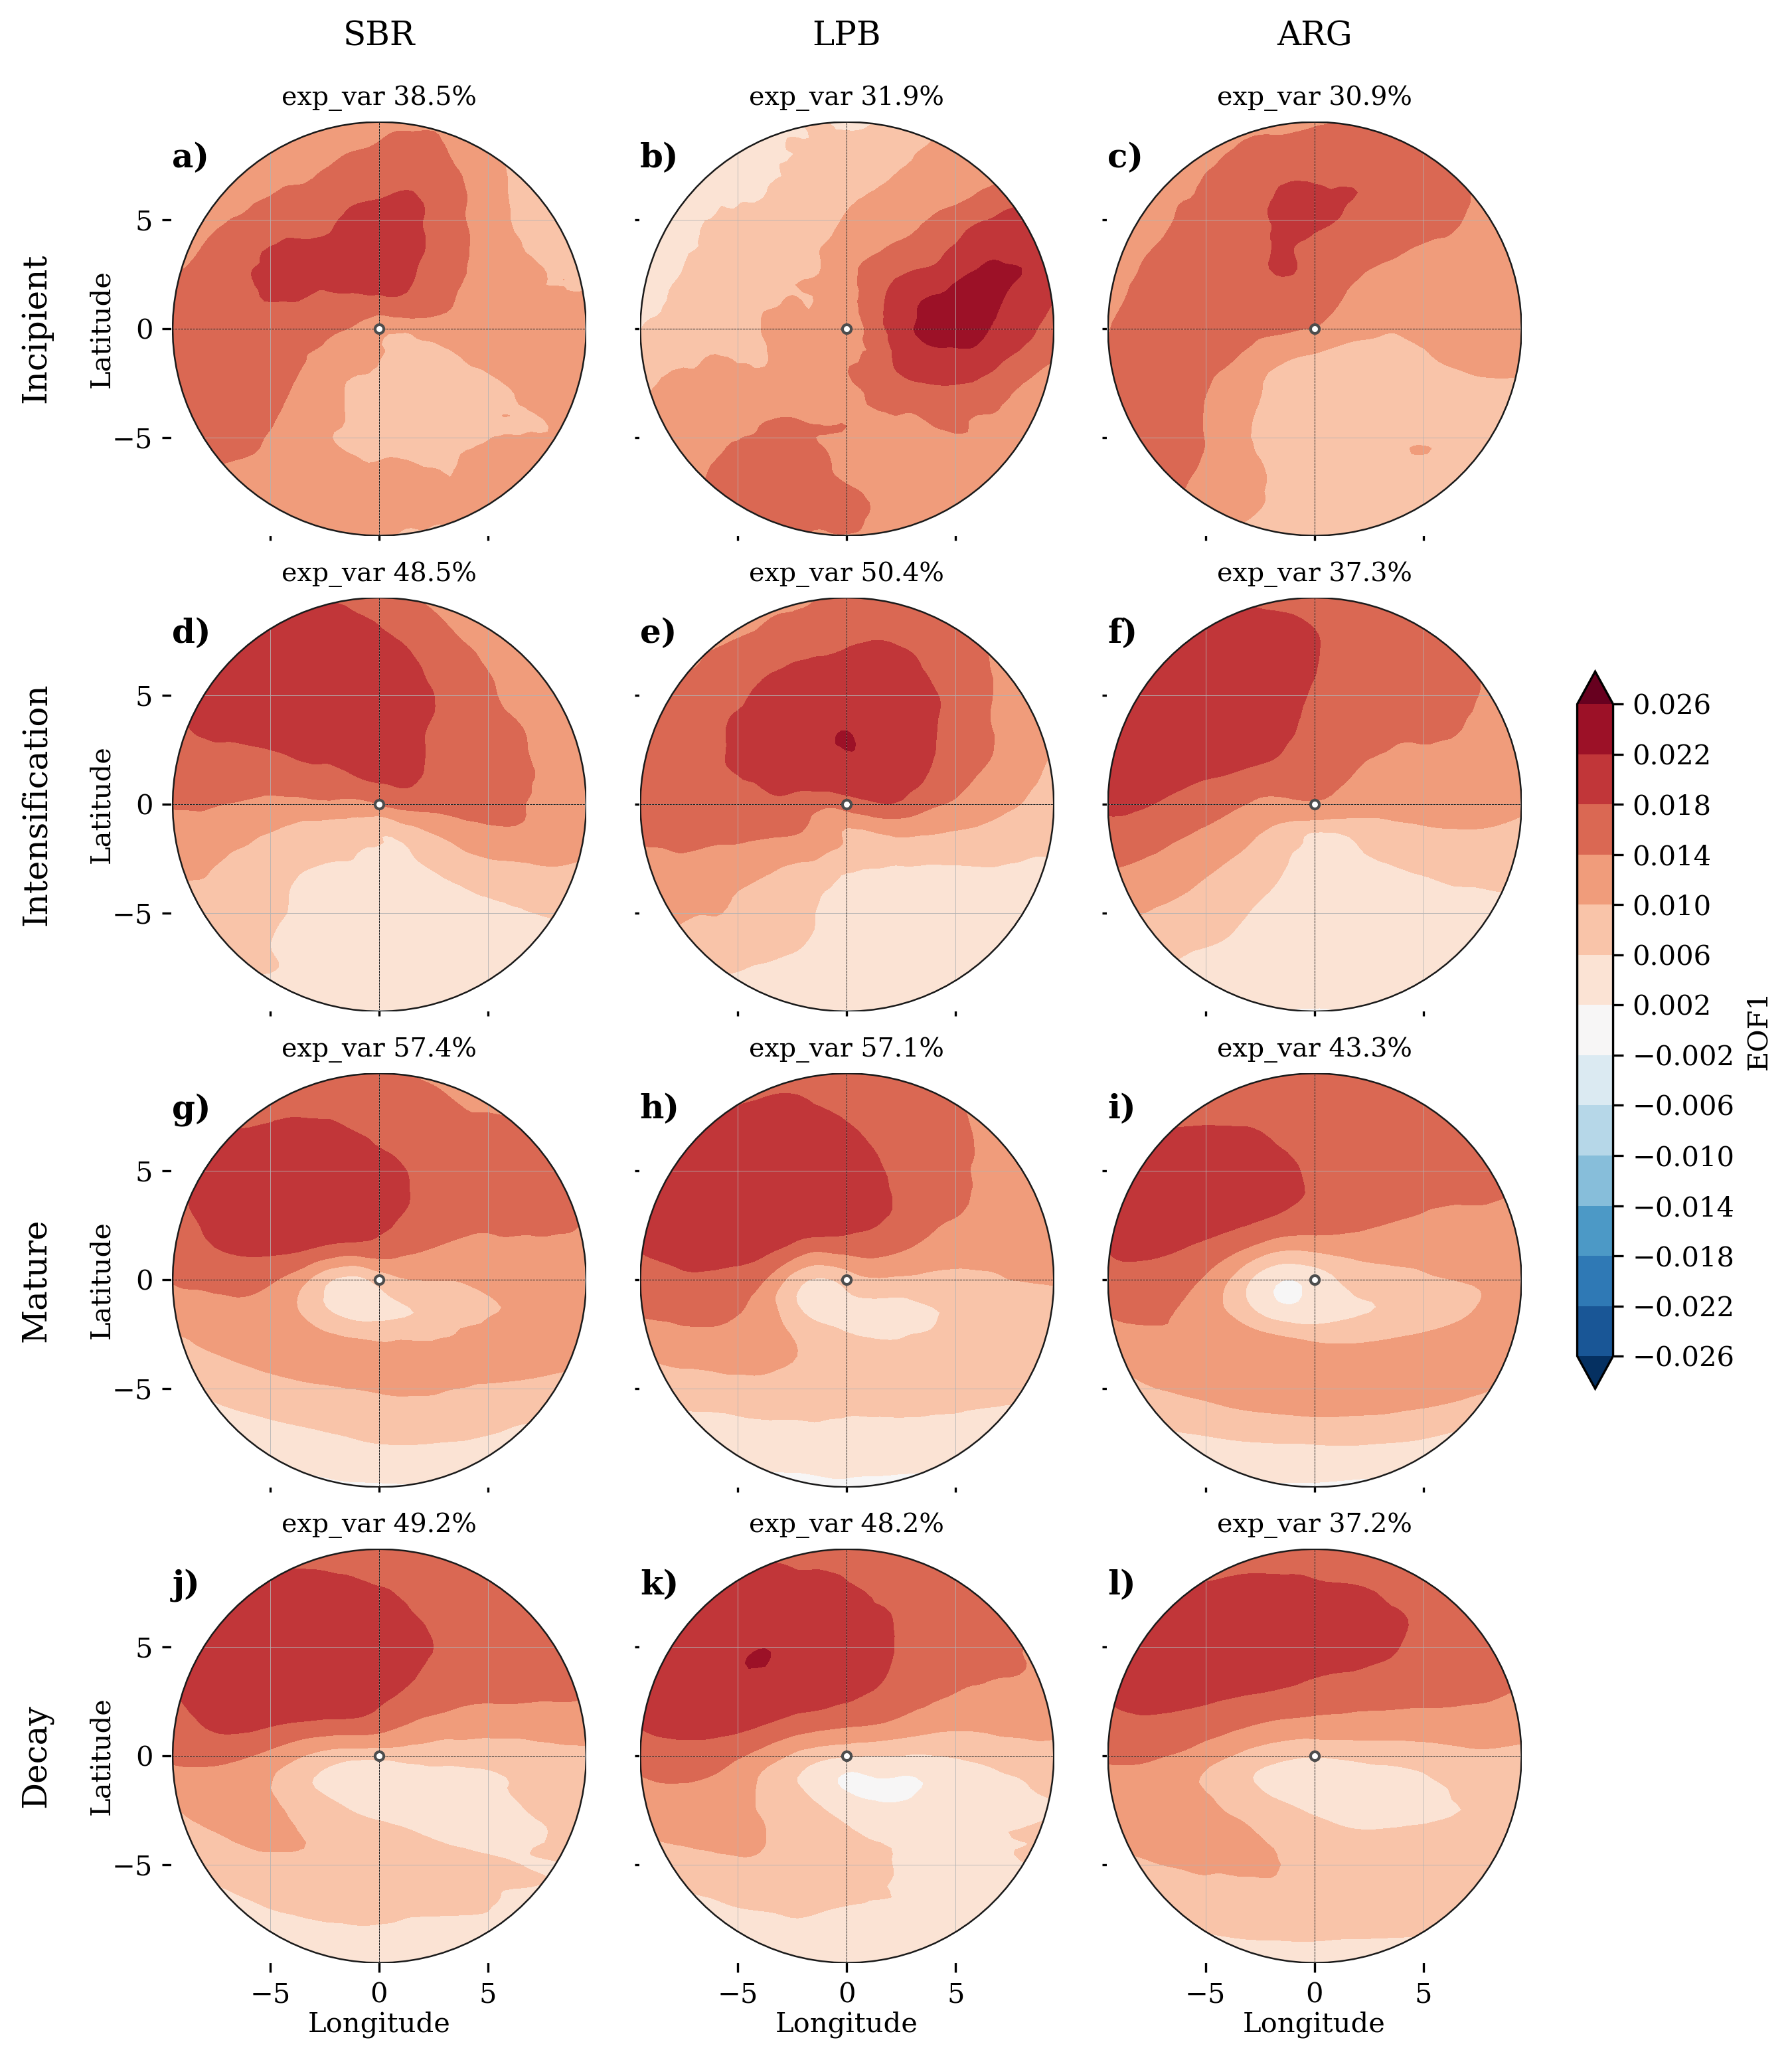
\includegraphics[width=\textwidth]{images/w10/pca1_wind10_global_fasesxreg.png}
\caption[EOF1 da magnitude do vento a 10 metros - População Global]{Primeiro modo espacial (EOF1) da magnitude do vento a 10 metros para a População Global de referência. Os painéis (a--c) correspondem à fase incipiente (Ic) para as regiões SBR, LPB e ARG, respectivamente; (d--f) à intensificação (It); (g--i) à maturidade (M); e (j--l) à decadência (D). O título de cada painel indica o percentual de variância explicada (\textit{exp\_var}) por este modo dominante. As cores quentes (frias) representam anomalias positivas (negativas) da estrutura do vento relativa ao centro do ciclone em um domínio de $20^{\circ} \times 20^{\circ}$.}
\label{fig:eof1_wind10_global}
\end{figure}

A Figura~\ref{fig:eof1_wind10_global} apresenta o primeiro modo das Funções Ortogonais Empíricas (EOF1) do campo de vento a 10 metros, obtido mediante a decomposição da variância total espacial sobre o domínio lagrangiano. 
Tal como se evidenciou no fracionamento de energia (Seção~\ref{sec:var_exp_wind10}), na População Global o padrão EOF1 domina amplamente a variância do sistema, exibindo valores que oscilam entre 31,9\% e 57,4\% segundo a região e fase. 
Morfologicamente, rege uma estrutura de grande escala onde as anomalias positivas dominam o quadrante norte e a periferia do domínio (tons vermelhos, $+0,01$ a $+0,02$), enquanto uma zona de anomalias negativas ou neutras concentra-se ao redor e ao sul do centro do vórtice (tons brancos--azuis claros). 
A região LPB em intensificação (e) mostra um padrão morfologicamente distinto, com um núcleo anômalo positivo centralizado. Finalmente, na fase de decadência (j, k, l), o dipolo homogeneiza-se e adota uma disposição estritamente zonal em todas as regiões, separando o domínio em uma metade norte negativa e uma metade sul fortemente positiva.

A presença deste dipolo norte-sul de grande escala, somado à sua alta variância explicada, indica que a principal fonte de variabilidade no vento dos ciclones típicos está ditada por sua interação com o fluxo zonal de fundo (os ventos do oeste de latitudes médias) e as flutuações do gradiente latitudinal de temperatura. 
Como detalha \citet{hannachi2007empirical}, a emergência de uma estrutura dipolar dominante (EOF1) constitui a assinatura matemática que representa o deslocamento posicional de uma corrente. 
Fisicamente, no Hemisfério Sul, isto traduz-se em deslocamentos da latitude relativa das correntes em jato na alta troposfera.
De acordo com \citet{hoskins2005new} e \citet{dossantos2023response}, a evolução estrutural dos ciclones ordinários depende fortemente deste acoplamento baroclínico profundo; portanto, as anomalias capturadas pela EOF1 refletem como o sistema expande ou contrai seu campo de vento em resposta à posição do jato. 

O fato de que as anomalias positivas deste dipolo concentrem-se marcadamente ao sul do centro (tons vermelhos em d, f, g, i) responde à assimetria térmica característica dos sistemas do Atlântico Sul. 
Tal como descrevem \citet{sinclair1997objective} e \citet{reboita2010south}, à medida que os ciclones se intensificam e ganham latitude, o gradiente horizontal de pressão tende a maximizar-se em seu setor austral devido à interação da circulação ciclônica com os anticiclones migratórios, acelerando os ventos nessa faixa. 
A exceção geométrica observada na região LPB (e) durante sua intensificação respalda esta dependência dos forçantes físicos: de acordo com \citet{gramcianinov2019properties}, os sistemas nesta zona estão fortemente modulados em suas etapas iniciais pela influência da baixa orográfica, o que gera uma variância do vento ancorada a forçantes topográficos centralizados, retardando temporalmente a imposição do dipolo zonal de grande escala. 
No decaimento, ao agotar-se a baroclinicidade e enfraquecer-se o vórtice, a circulação ciclônica perde definição e a variabilidade fica submetida aos deslocamentos do gradiente de pressão meridional do ambiente sinóptico.
A extração deste padrão univariado cumpre a função de estabelecer a linha de base de variabilidade estrutural para o ciclone extratropical médio. 

\subsubsection{Subconjunto p90}\label{subsubsec:eof1_wind10_p90}

\begin{figure}[htbp]
\centering
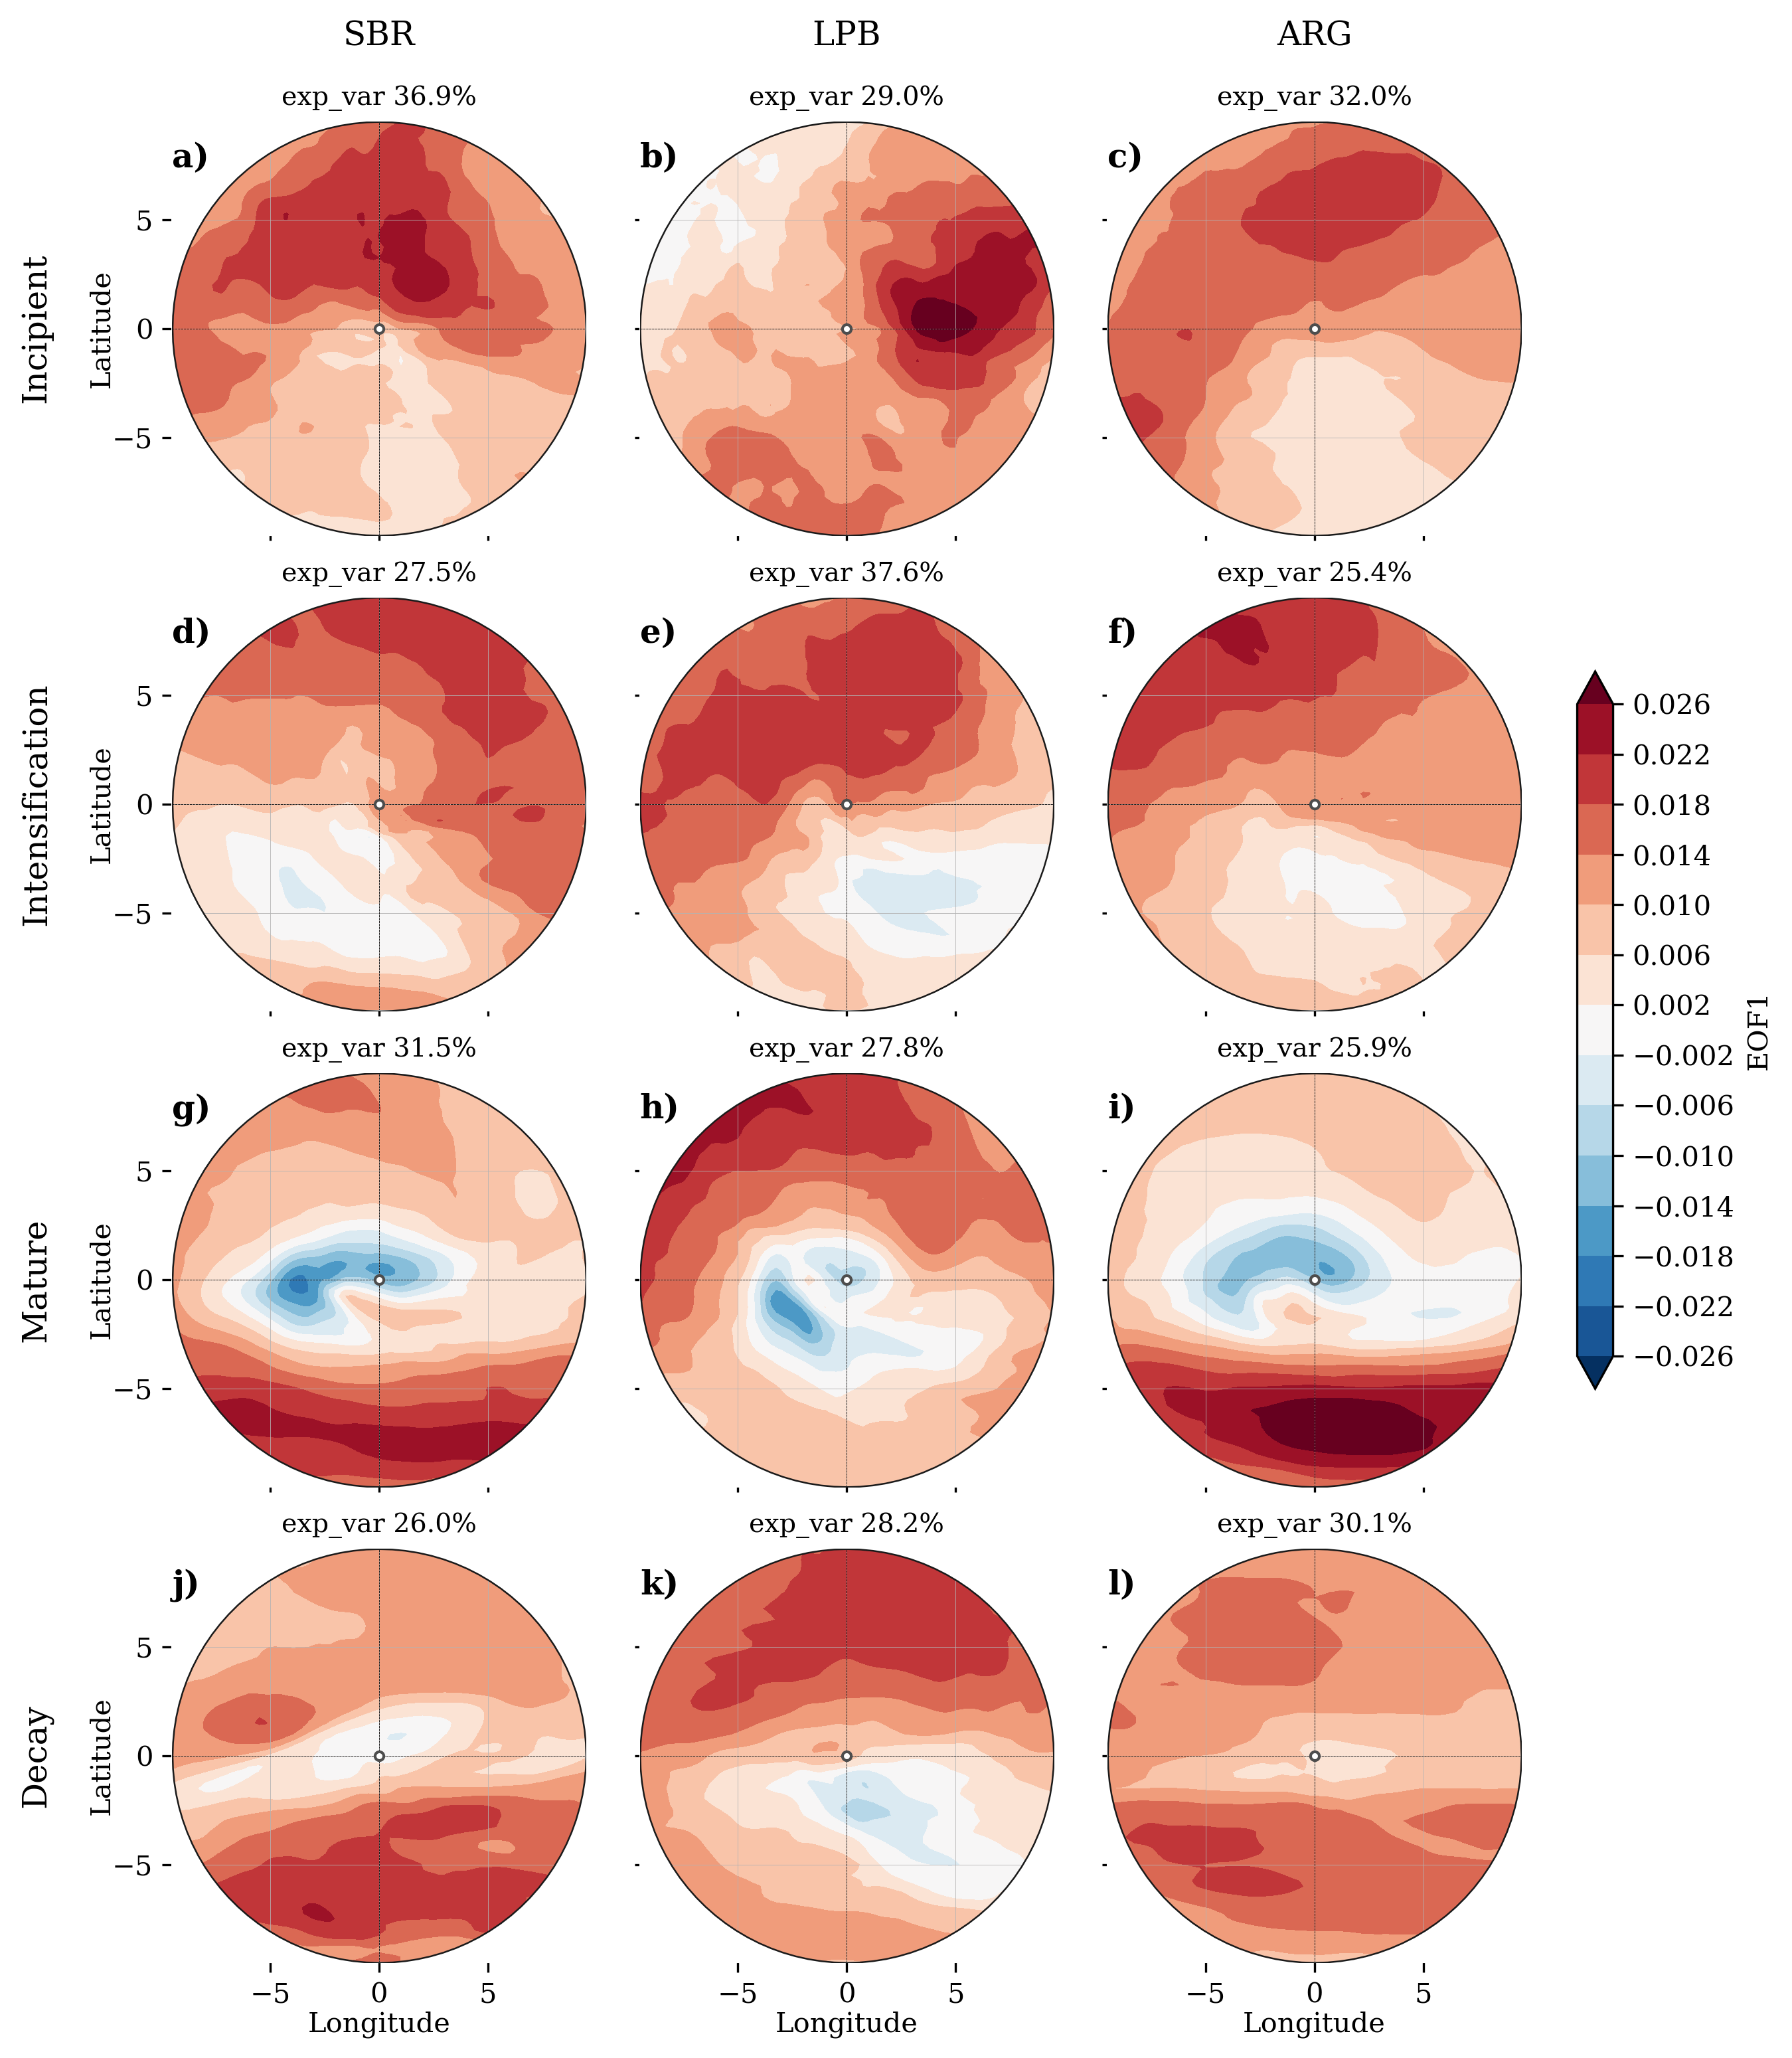
\includegraphics[width=\textwidth]{images/w10/pca1_wind10_p90_fasesxreg.png}
\caption[EOF1 da magnitude do vento a 10 metros - Subconjunto p90]{Primeiro modo espacial (EOF1) da magnitude do vento a 10 metros para o subconjunto de ciclones intensos (p90). A disposição dos painéis (a--l) por região de ciclogênese (colunas) e fase evolutiva (fileiras) é idêntica à Figura~\ref{fig:eof1_wind10_global}. Detalha-se a variância explicada (\textit{exp\_var}) em cada painel e a barra de cor padronizada para avaliar as diferenças nas assinaturas espaciais dos eventos intensos frente ao comportamento climatológico.}
\label{fig:eof1_wind10_p90}
\end{figure}

O contraste contra a organização dipolar da população geral revela que os ciclones intensos não amplificam linearmente o padrão base, mas reconfiguram radicalmente sua arquitetura modal. 
A Figura~\ref{fig:eof1_wind10_p90} ilustra que, em p90, a proporção de energia capturada pelo modo EOF1 reduz-se drasticamente, oscilando entre 25,4\% e 37,6\%, e sua topologia difere substancialmente ao mostrar assinaturas espacialmente complexas e hiperlocalizadas. 
Na fase de intensificação de SBR (d), emerge uma forte anomalia positiva que cobre a maior parte do domínio, com maior intensidade no norte e noroeste (vermelho escuro, $>+0,03$). 
Mais destacável é o comportamento na maturidade (g, h, i): LPB (h) exibe um dipolo fortemente inclinado com um núcleo negativo sumamente intenso e compacto ao sul do centro, rodeado por uma região de anomalias positivas que domina o setor norte e noroeste do domínio; ARG (i) desenvolve um padrão complexo onde a anomalia positiva cobre o norte e a periferia sul, com uma região de transição no centro. 
No decaimiento (j, k, l), embora retorne uma estrutura pseudozonal, os gradientes anômalos são notavelmente mais estreitos e confinados próximo ao núcleo em comparação com o relaxamento expansivo observado na população geral.

A quebra do padrão dipolar simples e a hiperlocalização das anomalias são a manifestação espacial da fragmentação de energia multiescalar discutida previamente.
Fisicamente, isto confirma que nestes eventos a intensa circulação fechada de mesoescala domina sobre o fluxo de fundo. 
O núcleo compacto e potente observado na maturidade de LPB (h) evidencia variabilidade na posição exata e severidade de estruturas mesoescalares. 
De acordo com o marco dinâmico documentado por \citet{clark2005sting} e \citet{han2025system} — e coerente com a localização espacial discutida na Seção~\ref{sec:kde_espacial_p90} —, a cinta transportadora fria (CCB) e os processos de fratura frontal rápida impulsionados por altas taxas de vorticidade traduzem-se modalmente em um EOF1 compacto e localizado, incapaz de ser capturado mediante um padrão de grande escala. 
Por outro lado, em ARG (i), o aparecimento de um padrão tripolar com uma anomalia negativa central durante a maturidade indica flutuações no tamanho da seclusão quente (\textit{warm seclusion}). 
Como detalham \citet{schultz2021antecedents} e \citet{reboita2022from}, a formação desta seclusão quente no núcleo, rodeada por um anel de ventos, é o traço evolutivo do modelo conceitual de Shapiro-Keyser, uma via de desenvolvimento característica de ciclones com alta organização baroclínica.

A quantificação destes modos revela que um ciclone intenso não é equivalente a um ciclone ordinário, mas que sua severidade dinâmica modifica a arquitetura do sistema. 
Como enfatizam \citet{corner2025classification} e \citet{eisenstein2023identification}, a severidade do vento não depende unicamente da sinótica, mas da manifestação destas características mesoescalares. 
% Identificar estas firmas asimétricas é clave para la meteorología en la prevision de estos eventos, ya que demuestra la variabilidad de los vientos más intensos, lo cual exige modelos de pronóstico capaces de resolver la dinámica estructural fina en los cuadrantes en relacion al centro del ciclón extratropical.

% ==============================================================================
\subsection{Significância estatística}\label{subsec:res_significancia_madurez}
% ==============================================================================

Para discriminar entre sinais físicos robustos e flutuações estocásticas próprias da reamostragem, avaliou-se a significância estatística dos autovetores espaciais mediante o método Bootstrap-$t$ (Seção \ref{subsec:bootstrap_significancia}). 
A Figura \ref{fig:xeof_madurez_global} documenta os três primeiros modos (EOF1--EOF3) e suas respectivas séries temporais (PC1--PC3) para a População Global em fase de maturidade, enquanto a Figura \ref{fig:xeof_madurez_p90} apresenta a análise equivalente para o subconjunto intenso $p90$.
O achurado delimita as áreas onde a EOF é estatisticamente significativa a 95\% de confiança.

\begin{figure}[htbp]
\centering
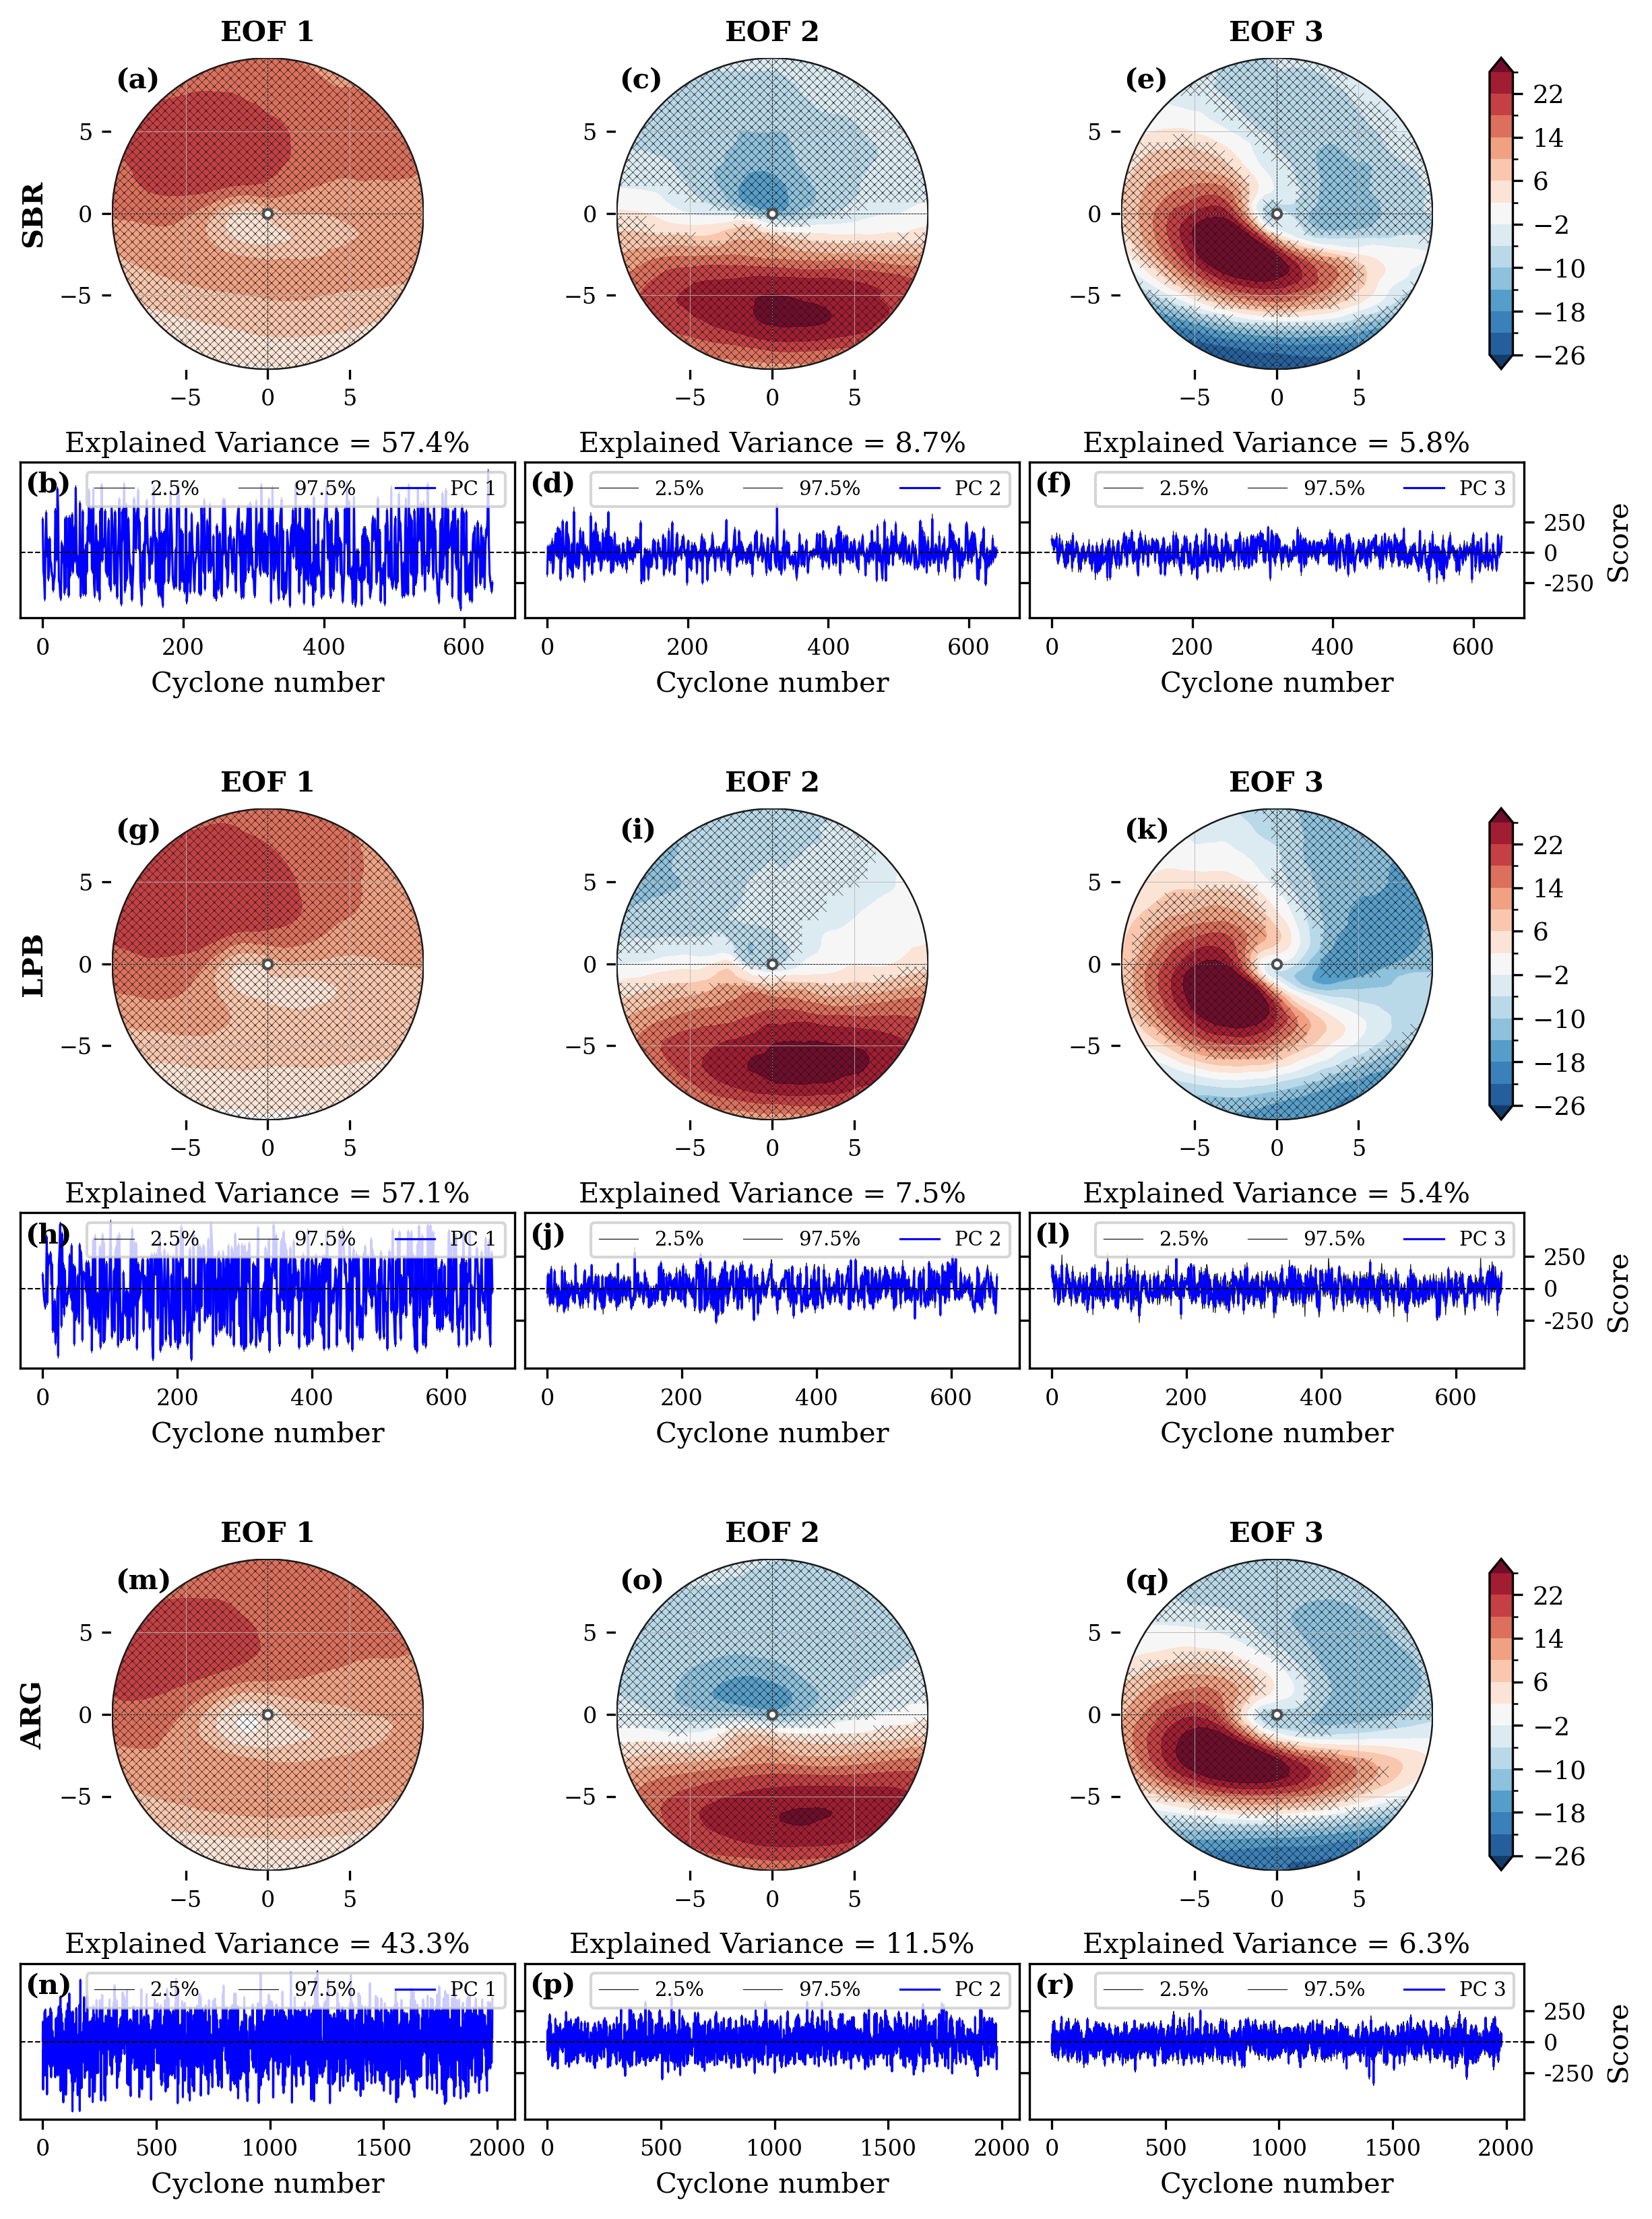
\includegraphics[width=\textwidth]{images/w10/xeof_global_wind10_mature.png}
\caption[Significância espacial dos EOFs em fase de maturidade - População Global]{Decomposição EOF do vento a 10 m para a População Global em fase de maturidade. Painéis (a, c, e): mapas dos três primeiros modos espaciais (EOF1--EOF3) com achurado indicando significância estatística a 95\% (teste Bootstrap-$t$). Painéis (b, d, f): séries temporais correspondentes das Componentes Principais (PC1--PC3). A linha cinza delimita os percentis 2,5 e 97,5 da distribuição bootstrap.}
\label{fig:xeof_madurez_global}
\end{figure}

\begin{figure}[htbp]
\centering
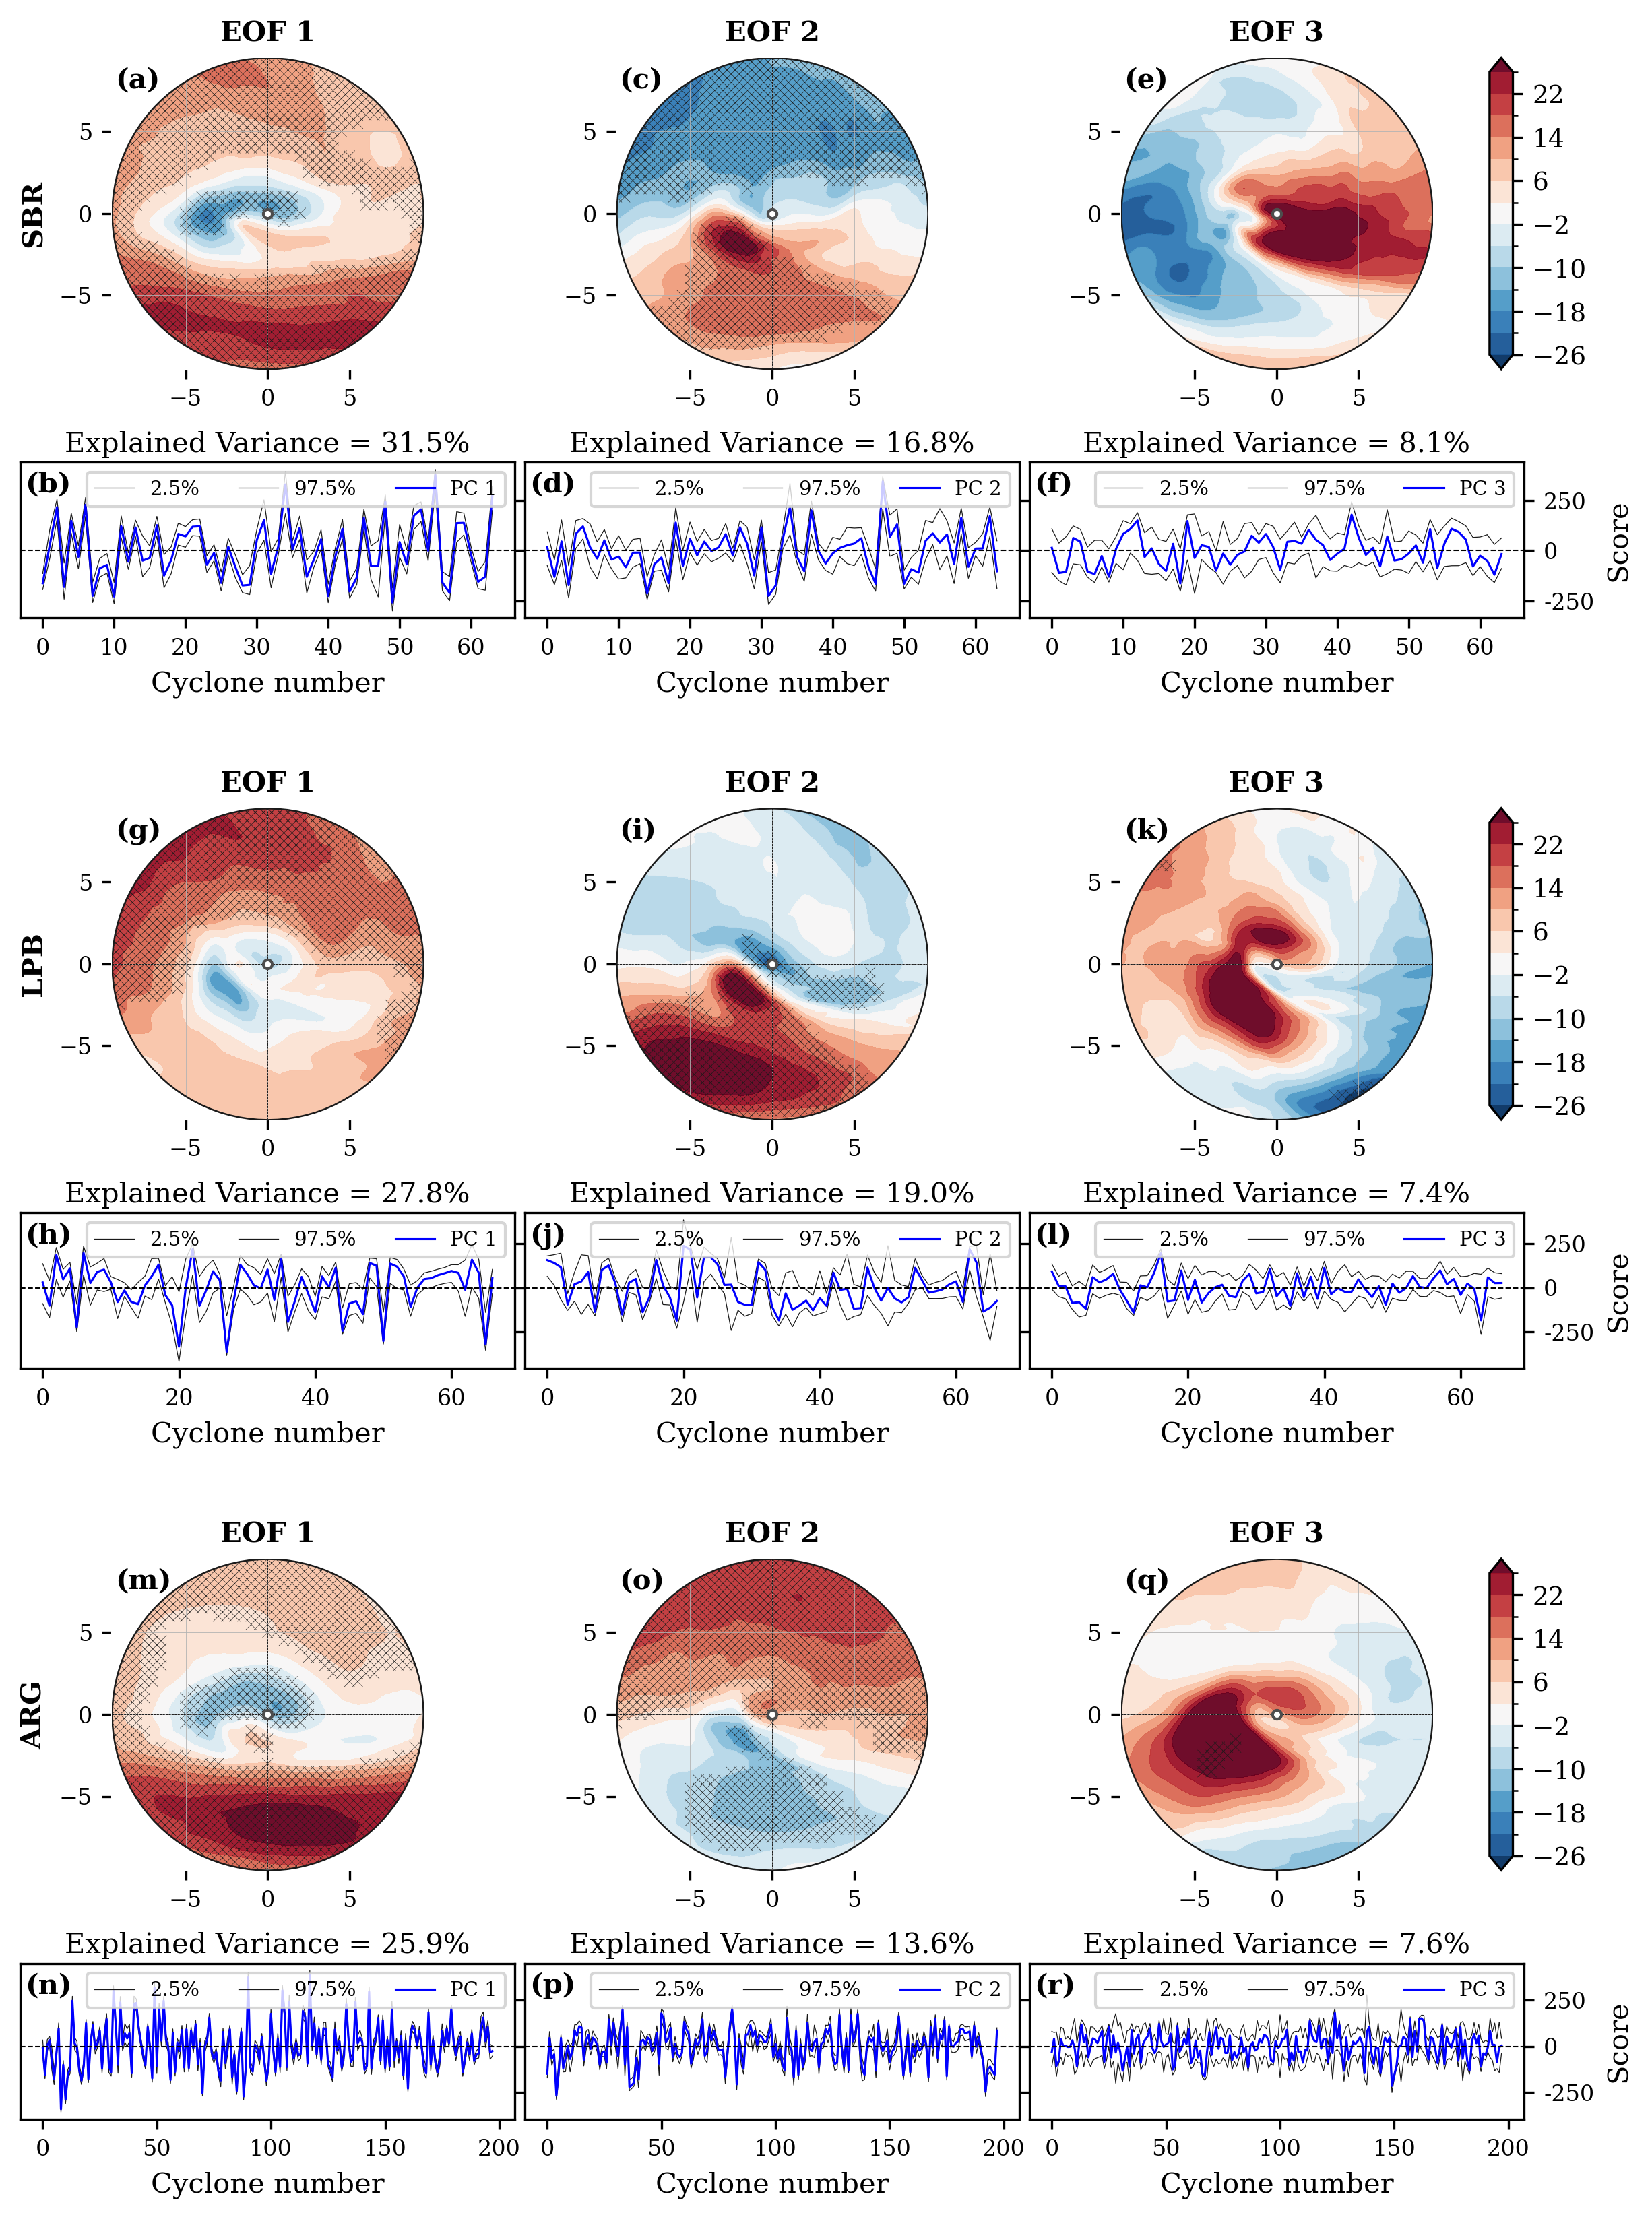
\includegraphics[width=\textwidth]{images/w10/xeof_p90_wind10_mature.png}
\caption[Significância espacial dos EOFs em fase de maturidade - Subconjunto p90]{Decomposição EOF do vento a 10 m para o subconjunto intenso ($p90$) em fase de maturidade. A disposição de painéis é idêntica à Figura \ref{fig:xeof_madurez_global}.}
\label{fig:xeof_madurez_p90}
\end{figure}

Na População Global (Figura \ref{fig:xeof_madurez_global}), o modo dominante (EOF1) exibe áreas de significância estatística que abrangem praticamente todo o domínio, particularmente nos setores norte e sul onde se localizam os máximos do dipolo baroclínico (painéis a, g, m). 
Esta extensão espacial da significância indica que o padrão dipolar não é um artefato da amostra, mas uma característica física estável e reprodutível dos ciclones maduros. 
Consistente com o alto percentual de variância explicada (43--57\%), as séries de PC1 (painéis b, h, n) mostram amplitudes que oscilam amplamente e dominam sobre as flutuações de PC2 e PC3, as quais permanecem confinadas dentro dos limites de confiança (linhas cinzas) e representam meramente ruído de fundo ou variabilidade intra-sistêmica menor.

Pelo contrário, no subconjunto $p90$ (Figura \ref{fig:xeof_madurez_p90}), as áreas significativas do EOF1 experimentam uma dramática contração para núcleos compactos próximos ao centro do vórtice (painéis a, g, m). 
Em SBR e LPB, a significância restringe-se a pequenos \textit{patches} ao redor do núcleo e do flanco sul, enquanto em ARG o padrão tripolar apresenta significância unicamente no anel periférico sul. 
Esta contração espacial confirma que, em ciclones intensos, o modo dominante perde coerência espacial fora do núcleo imediato; a estrutura do vento já não está governada por um gradiente sinóptico estendido, mas por processos de mesoescala localizados (seclusões térmicas, jatos de baixo nível) que variam substancialmente entre eventos individuais.

Mais crítico ainda é o comportamento das séries temporais no grupo $p90$ (painéis b, d, f e h, j, l). Diferentemente do grupo Global onde PC2 e PC3 são residuais, aqui as amplitudes de PC2 (linha azul em painéis d, j) e PC3 (painéis f, l) apresentam magnitudes comparáveis às de PC1 e com frequência superam os limites de confiança de 95\%, cruzando os limites de confiança de maneira sistemática. 
Isto demonstra estatisticamente que os modos secundários deixaram de ser ``ruído'' para converter-se em portadores de variância física significativa. 
A competição energética entre múltiplos PCs reflete a fragmentação dinâmica do campo de vento: quando um ciclone é intenso, sua estrutura cinemática já não pode ser descrita mediante um único padrão espacial dominante, mas requer a superposição de vários modos ortogonais competitivos.

A contração das áreas significativas no grupo $p90$ indica que a preditibilidade espacial do campo de vento reduz-se drasticamente nestes ciclones. 
Enquanto em sistemas ordinários podemos confiar de que o padrão dipolar estendido representará fielmente a distribuição de ventos, em sistemas severos somente o núcleo imediato do vórtice apresenta um sinal robusto; os flancos e quadrantes periféricos estão dominados por variabilidade estocástica ou estruturas transitórias de mesoescala que escapam ao primeiro modo. 

% ==============================================================================
\section{Componentes principais (PC1)}\label{subsec:res_dinamica_pc1}

A fragmentação da variância e a contração das áreas significativas observadas na fase de maturidade (Seção \ref{subsec:res_significancia_madurez}) têm sua contraparte temporal no comportamento estatístico das Componentes Principais. 
Enquanto na População Global a PC1 domina estavelmente a evolução do sistema — evidenciado por suas amplitudes superiores e áreas significativas extensas —, nos ciclones intensos a competição entre múltiplos modos ortogonais (Figura \ref{fig:xeof_madurez_p90}) traduz-se em propriedades estatísticas distintivas: uma correlação fraca com o forçante sinóptico.

\input{tabelas_pt/tab_momentos_global_w10.tex}

\subsubsection{População Global: Padrão sinóptico dominante}

As Tabelas \ref{tab:momentos_global_w10} e \ref{tab:corr_global_w10} documentam as métricas estatísticas da PC1 para a População Global. Ao avaliar a evolução da população média, a distribuição da PC1 exibe uma progressiva \textit{normalização} estrutural. 
Nas três regiões (SBR, LPB e ARG), os valores de curtose oscilam de forma consistente entre $-0,30$ e $-1,03$ durante a intensificação e maturidade, evidenciando distribuições platicúrticas sem caudas extremas dominantes. 
Notavelmente, o regime transicional de LPB mostra a maior variabilidade inicial (\textit{skewness} $+0,99$, leptocurtose $+1,32$ em fase incipiente), enquanto SBR e ARG apresentam populações mais homogêneas desde etapas precoces.
O traço evolutivo mais contundente emerge no acoplamento com a vorticidade: em todas as regiões, a correlação inicial — que oscila entre $-0,35$ (LPB) e $-0,57$ (SBR) — experimenta um \textit{fortalecimento sistemático} até alcançar seu máximo na maturidade ($-0,890$ em SBR, $-0,868$ em LPB e $-0,860$ em ARG), caindo levemente durante o decaimento ($\rho < -0,75$).

\input{tabelas_pt/tab_corr_global_w10.tex}

Este acoplamento quase linear (que explica até $r^2 \approx 0,79$ da variância em SBR) demonstra que, nos ciclones ordinários, a variabilidade espacial do vento está governada diretamente pelo gradiente de pressão em escala sinóptica. 
A progressiva simetrização da distribuição de PC1 (\textit{skewness} tendendo a zero) evidencia que, à medida que o vórtice se intensifica, os campos de vento convergem para uma configuração prototípica, dominada pelo primeiro modo de variabilidade. 
Então, para a maioria dos ciclones, a estrutura espacial do vento não é arbitrária, mas organiza-se em torno de um padrão coerente (EOF1). 
A severidade extrema rompe tal organização, permitindo que o sistema explore múltiplas configurações espaciais válidas.
A diferença entre regiões reside na velocidade desta convergência: enquanto SBR exibe um acoplamento forte desde etapas incipientes, LPB requer a fase de intensificação para alcançar tal estado (passando de $\rho = -0,35$ a $-0,71$), refletindo seu caráter transicional onde a organização frontal emerge somente quando o forçante baroclínico se estabelece com suficiente intensidade.
% Establecer esta línea base cinemática es importante para validar estadísticamente que los modelos de gran escala representan la mayoría de los ciclones. 
Em sistemas de intensidade regular (População Global), é possível inferir com confiança o padrão espacial da circulação superficial observando unicamente a vorticidade relativa em 850 hPa.

\subsubsection{Subconjunto ($p90$): Desacoplamento estrutural}

As Tabelas \ref{tab:momentos_p90_w10} e \ref{tab:corr_p90_w10} expõem os parâmetros estatísticos para o grupo de ciclones mais intensos (p90). 
A dinâmica dos eventos intensos rompe drasticamente com a linearidade observada na População Global. 
Em vez de intensificar-se para a maturidade, a correlação entre PC1 e vorticidade exibe um colapso estrutural nas regiões baroclínicas: em ARG cai progressivamente desde $-0,43$ (incipiente) até um mínimo de $-0,26$ em maturidade, enquanto LPB e SBR mostram correlações estagnadas ou em descenso ($-0,37$ e $-0,44$, respectivamente). 
Este colapso correlacional é consistente com a perda de significância espacial observada no modo dominante (Figura \ref{fig:xeof_madurez_p90}, painéis a, g, m): quando o padrão espacial somente é robusto no núcleo imediato do vórtice mas não nos flancos (como documentou o teste Bootstrap-$t$ na seção anterior), sua amplitude temporal (PC1) deixa de escalar coerentemente com a intensidade ($\zeta_{850}^{min}$).

\input{tabelas_pt/tab_momentos_p90_w10.tex}

Paralelamente, as distribuições de probabilidade revelam uma \textit{heterogeneização} marcada. 
LPB exibe leptocurtose ($\gamma_2 = +0,96$) e forte assimetria negativa ($\gamma_1 = -0,88$) durante a intensificação, indicando uma população bimodal de configurações estruturais. 
SBR, por sua parte, mantém estabilidade durante o desenvolvimento mas exibe uma bifurcação extrema no decaimento: uma leptocurtose ($\gamma_2 = +3,95$) com \textit{skewness} positivo ($+1,15$), evidenciando que os ciclones intensos não seguem um único caminho estrutural para a dissipação.
Esta queda correlacional é a expressão quantitativa do desacoplamento mesoescalar já evidenciado espacialmente na Seção~\ref{subsec:res_significancia_madurez}. 
Quando um ciclone se aprofunda, a organização do vento a 10 metros deixa de obedecer puramente ao mínimo de vorticidade e passa a ser controlada por processos secundários: gênese de seclusões quentes em ARG, organização convectiva profunda independente em SBR, ou interações orográficas persistentes em LPB. 

A emergência de curtose positiva em LPB (intensificação/maturidade) e SBR (decaimento) demonstra que a severidade alcança-se através de uma \textit{diversidade de estruturas assimétricas} que o modo dominante não captura. 
Sorpreendentemente, o acoplamento somente se recupera abruptamente durante o decaimento (alcançando $-0,74$ em ARG), sugerindo que, uma vez dissipadas as anomalias térmicas de mesoescala (atrito e perda de gradiente), a circulação remanescente volta a alinhar-se linearmente com o vórtice residual.

\input{tabelas_pt/tab_corr_p90_w10.tex}

Este achado quantitativo prova que alcançar a severidade dinâmica máxima induz um \textit{desacoplamento temporal} entre o campo de vento superficial e a vorticidade do ciclone durante a fase de maturidade.
Isto indica que parametrizar a evolução cinemática de um ciclone severo utilizando unicamente $\zeta_{850}$ resultará insuficiente no momento crítico de ocorrência, já que a distribuição dos ventos obedece a alterações internas de mesoescala que escapam da linearidade sinóptica. 

\section{Síntese}\label{sec:sintesis_wind10}

Na População Global, o vento superficial organiza-se como uma resposta passiva ao forçante baroclínico sinóptico: as PDFs mostram distribuições unimodais estreitas, os máximos dispersam-se amplamente no domínio lagrangiano (KDE difuso), e a variância espacial concentra-se em um único modo dipolar (EOF1) que escala coerentemente com a vorticidade relativa ($\rho < -0,85$ em maturidade). 
Em contraste, os sistemas intensos (p90) exibem uma arquitetura cinemática qualitativamente diferente. 
A transição para a maturidade gera: 
(i) caudas estendidas nas PDFs alcançando 30 m s$^{-1}$ com modas deslocadas para 20--25 m s$^{-1}$; 
(ii) uma hiperconcentração espacial dos máximos no quadrante noroeste (Hemisfério Sul), coerente com a dinâmica da cinta transportadora fria e processos de fratura frontal; e 
(iii) uma fragmentação da variância entre múltiplos modos ortogonais (EOF1--EOF3), onde o modo dominante perde significância espacial fora do núcleo imediato e sua amplitude (PC1) desacopla-se da intensidade sinóptica ($\rho \approx -0,26$ a $-0,44$). 

Em ciclones não intensos o campo de vento pode ser inferido linearmente desde a vorticidade mínima, enquanto que, em sistemas severos a distribuição de ventos máximos obedece a processos de mesoescala — seclusões térmicas, descargas descendentes e jatos de baixo nível — que exigem diagnósticos adicionais (estabilidade estática, umidade em setores quentes) durante a fase crítica de maturidade. 
As diferenças regionais modulam essas tendências gerais. 
Os sistemas originados em SBR e LPB desenvolvem núcleos de vento mais intensos e coerentes, favorecidos por fluxos de calor latente oceânico e configurações orográficas que organizam a convecção, enquanto os ciclones de ARG apresentam maior heterogeneidade estrutural.

O estabelecimento desta base — que vincula a severidade (p90) com uma organização espacial específica e previsível do vento máximo — constitui o ponto de partida para avaliar a relação com outros campos de variáveis como a precipitação. 
Esta integração multivariada pode aportar conhecimento desde o paradigma dos eventos compostos; assim como mostra a investigação de \citet{zscheischler2018future}, onde a concorrência espacial e temporal de múltiplos perigos físicos produz impactos socioeconômicos substancialmente maiores aos de cada variável atuando de forma isolada.